\documentclass[aspectratio=169,10pt]{beamer}
\def\animbuild{0} % 1 = animaciones
% Estilo de la presentación del TP3

\usepackage[T1]{fontenc}
\usepackage[utf8]{inputenc}
\usepackage[spanish,es-noshorthands,es-nodecimaldot]{babel}


\usepackage{lmodern}
\usefonttheme{professionalfonts}
\usepackage{mathptmx}
\usepackage{amsmath,amssymb}
\DeclareSymbolFont{symbols}{OMS}{cmsy}{m}{n}
\SetSymbolFont{symbols}{bold}{OMS}{cmsy}{b}{n}
\DeclareSymbolFontAlphabet{\mathcal}{symbols}

\usepackage{graphicx}
\usepackage{tikz}
\usetikzlibrary{arrows.meta,positioning}
\graphicspath{{images/}{../data/}}

\usetheme{Warsaw}
\setbeamertemplate{navigation symbols}{}
\definecolor{acento}{rgb}{0.2,0.2,0.7} 

\setbeamertemplate{headline}{%
  \leavevmode%
  \hbox{%
    \begin{beamercolorbox}[wd=\paperwidth,ht=2.6ex,dp=1.3ex,leftskip=.3cm,rightskip=.3cm]{section in head/foot}%
      \usebeamerfont{section in head/foot}%
      \insertsectionnavigationhorizontal{.98\paperwidth}{}{\hskip0pt plus1filll}%
    \end{beamercolorbox}%
    \begin{beamercolorbox}[wd=\paperwidth,ht=2.2ex,dp=1ex,leftskip=.3cm,rightskip=.3cm]{subsection in head/foot}%
      \usebeamerfont{subsection in head/foot}%
      \insertsubsectionnavigationhorizontal{.98\paperwidth}{}{\hskip0pt plus1filll}%
    \end{beamercolorbox}%
  }%
  \vskip0pt%
}

% Sin esto las diapositivas salen sin numerar.
\setbeamertemplate{page number in head/foot}[framenumber]

% Separador con el título de la sección, sin numerar.
\AtBeginSection[]{%
  \begin{frame}[plain,noframenumbering]
    \vfill\centering\usebeamercolor[fg]{structure}%
    {\Huge\bfseries\insertsectionhead}\vfill
  \end{frame}%
}


\newcommand{\vv}[1]{\mathbf{#1}}
\newcommand{\ten}[1]{\times 10^{#1}}
\newcommand{\uni}[1]{\,\mathrm{#1}}
\newcommand{\va}{v_{a}}

\newcommand{\siimagen}[3]{%
  \IfFileExists{images/#1}{#2}{%
    \IfFileExists{../data/#1}{#2}{%
      \IfFileExists{figs/#1}{#2}{#3}}}%
}

\newcommand{\figura}[2][\linewidth]{%
  \siimagen{#2}%
    {\makebox[\linewidth][c]{\includegraphics[width=#1,height=0.74\textheight,keepaspectratio]{#2}}}%
    {\makebox[\linewidth][c]{\framebox[#1][c]{\rule{0pt}{5cm}\textit{falta la figura}}}}%
}


\newenvironment{cols}{\begin{columns}[c]}{\end{columns}}

\newenvironment{resultado}[1][Resultado]{%
  \begin{beamercolorbox}[wd=\linewidth,sep=6pt,rounded=true]{block body alerted}%
  \footnotesize\textbf{#1}\par\vspace{2pt}%
  \begin{itemize}\setlength{\itemsep}{1pt}%
}{%
  \end{itemize}\end{beamercolorbox}%
}

\newenvironment{parametros}[1][Parámetros]{%
  \begin{beamercolorbox}[wd=\linewidth,sep=6pt,rounded=true]{block body}%
  \footnotesize\textbf{#1}\par\vspace{2pt}%
  \begin{itemize}\setlength{\itemsep}{1pt}%
}{%
  \end{itemize}\end{beamercolorbox}%
}

\providecommand{\animbuild}{0}
\newif\ifanim
\ifnum\animbuild=1 \animtrue \else \animfalse \fi
\ifanim\usepackage{animate}\fi

\newcommand{\animacion}[6]{%
  \ifanim
    \animategraphics[autoplay,loop,width=\linewidth]{#4}{#1}{#2}{#3}%
  \else
    \siimagen{#5}%
      {\makebox[\linewidth][c]{\includegraphics[width=\linewidth,height=0.88\textheight,keepaspectratio]{#5}}}%
      {\makebox[\linewidth][c]{\framebox[\linewidth][c]{\rule{0pt}{4.2cm}\textit{fotograma}}}}%

    \if\relax\detokenize{#6}\relax\else
      \par\vspace{2pt}{\scriptsize\color{acento}\url{#6}}%
    \fi%
  \fi
}


% Logo ITBA al pie de la portada
\addtobeamertemplate{title page}{}{%
  \begin{tikzpicture}[remember picture,overlay]
    \node[
      anchor=south,
      yshift=0.35cm
    ] at (current page.south) {%
      
\includegraphics[height=0.65cm]{images/Itba_bsas_logo.png}
    };
  \end{tikzpicture}%
}
% Generado por python/dcm_report.py (docs/results/1.3/cortes.txt). No editar a mano.
\newcommand{\DcmDvacia}{0.0093 \pm 0.0014}
\newcommand{\DcmCortevacia}{6}
\newcommand{\DcmRangovacia}{0.0077\text{--}0.0108}
\newcommand{\DcmDdiscochico}{0.0032 \pm 0.0007}
\newcommand{\DcmCortediscochico}{20}
\newcommand{\DcmRangodiscochico}{0.0037\text{--}0.0046}
\newcommand{\DcmDdiscogrande}{0.0020 \pm 0.0002}
\newcommand{\DcmCortediscogrande}{10}
\newcommand{\DcmRangodiscogrande}{0.0015\text{--}0.0024}
\newcommand{\DcmDparedA}{0.0030 \pm 0.0005}
\newcommand{\DcmCorteparedA}{4}
\newcommand{\DcmRangoparedA}{0.0030\text{--}0.0035}
\newcommand{\DcmDparedB}{0.0019 \pm 0.0003}
\newcommand{\DcmCorteparedB}{9}
\newcommand{\DcmRangoparedB}{0.0016\text{--}0.0023}
\newcommand{\DcmDparedC}{0.0014 \pm 0.0003}
\newcommand{\DcmCorteparedC}{8}
\newcommand{\DcmRangoparedC}{0.0015\text{--}0.0017}
\newcommand{\DcmDejemplo}{0.0098}
\newcommand{\DcmMesetavacia}{0.284 \pm 0.015}

\usepackage{caption}
\usepackage{media9}
\hypersetup{colorlinks=true, urlcolor=blue, linkcolor=blue}
\usepackage{algorithm}
\usepackage{algpseudocode}
\newif\ifshowvideo 
\showvideotrue
%% cambiar para mostrar las animaciones embebdidas o los stills$$

\title[TP3]{Trabajo Práctico Nro. 3: Simulación Dirigida por Eventos}
\subtitle{Colisiones entre partículas}
\author[Grupo 03]{Matías Leporini \and Camila Lee \and Ana Negre}
\institute{
Instituto Tecnológico de Buenos Aires (ITBA)\\
72.25 - Simulación de Sistemas
}
\date{28 de septiembre de 2026}

\begin{document}

\begin{frame}[plain,noframenumbering]
  \titlepage
\end{frame}

\section{Introducción}

\begin{frame}{Modelo}
  \begin{columns}[T]
    \begin{column}{0.48\textwidth}
      \textbf{Partículas}\par\vspace{4pt}
      \setlength{\abovedisplayskip}{0pt}\setlength{\abovedisplayshortskip}{0pt}
      \begin{align*}
        \vv{r}_i(t+t_c) &= \vv{r}_i(t) + \vv{v}_i(t)\,t_c \\[2pt]
        \vv{v}_i((t+t_c)^-) &= \vv{v}_i(t) \\[4pt]
        \|\vv{r}_j-\vv{r}_i\| &= r_i+r_j
      \end{align*}
      {\footnotesize $t_c$: tiempo hasta el próximo evento.}
    \end{column}
    \begin{column}{0.50\textwidth}
    
      \textbf{Colisiones}\par\vspace{4pt}
      \setlength{\abovedisplayskip}{0pt}\setlength{\abovedisplayshortskip}{0pt}
      \begin{align*}
        \vv{v}_i' &= \vv{v}_i + \frac{J}{m_i}\,\vv{n} \\[2pt]
        \vv{v}_j' &= \vv{v}_j - \frac{J}{m_j}\,\vv{n} \\[2pt]
        J &= \frac{2m_i m_j}{m_i+m_j}
        (\vv{v}_j-\vv{v}_i)\cdot\vv{n}
      \end{align*}
      \vspace{-2pt}
      {\footnotesize
      $\vv{n}=(\vv{r}_j-\vv{r}_i)/(r_i+r_j)$: normal de contacto.\\
      Choques elásticos e instantáneos.}
    \end{column}
  \end{columns}
\end{frame}

\section{Implementación}

\begin{frame}{Arquitectura del motor}
  \centering
  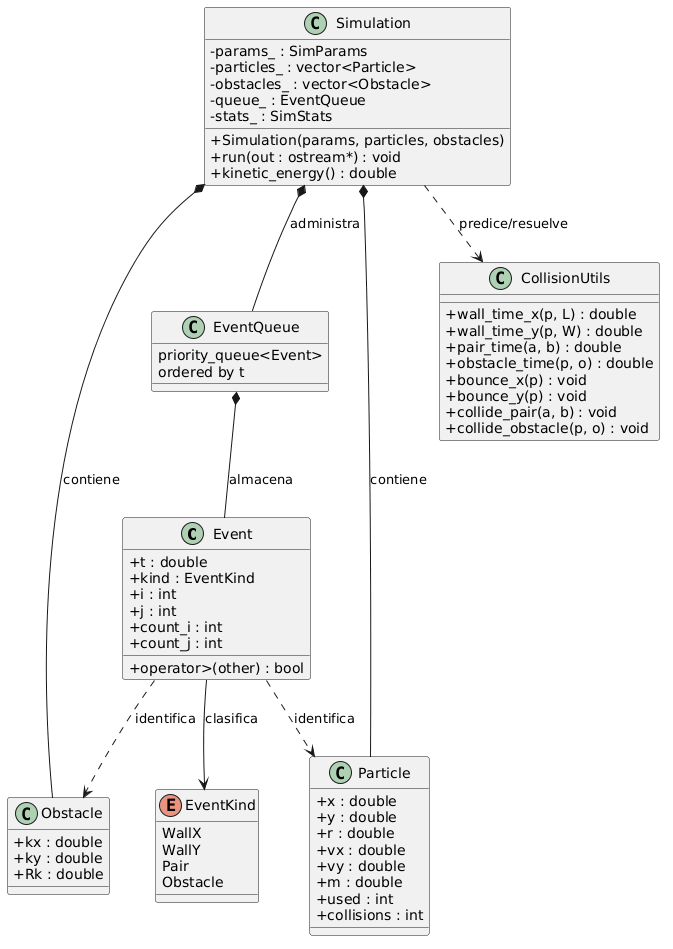
\includegraphics[width=\textwidth,height=0.86\textheight,keepaspectratio]{images/uml.png}
  \par\vspace{1pt}
  {\footnotesize Motor en C++. Cola con prioridad por tiempo de evento.}
\end{frame}

\begin{frame}{Simulación}
  \scriptsize
  \begin{algorithmic}[1]
    \State Inicializar $t$, partículas y cola de eventos $Q$
    \While{$Q \neq \emptyset$ y $\Call{top}{Q}.t \leq t_{\max}$}
      \State $e \gets \Call{pop}{Q}$
      \If{\Call{válido}{$e$}}
        \State Avanzar todas las partículas hasta $e.t$
        \State Resolver $e$ y actualizar velocidades
        \State Actualizar estadísticas y goles
        \State Recalcular eventos de las partículas afectadas
      \Else
        \State Descartar $e$ (predicción obsoleta)
      \EndIf
    \EndWhile
  \end{algorithmic}
\end{frame}

\section{Simulaciones}

\begin{frame}{Sistema particular simulado}
  \begin{cols}
    \begin{column}{0.44\textwidth}
      \centering
      \figura{system.png}
    \end{column}
    \begin{column}{0.52\textwidth}
      \begin{parametros}[Parámetros fijos]
        \item $L=1.20\,\mathrm{m}$
        \item $W=0.68\,\mathrm{m}$
        \item $d=0.20\,\mathrm{m}$
        \item $r = 0.0175\,\mathrm{m}$, radio partículas 
        \item $m = 0.025\,\mathrm{kg}$, masa partículas
        \item $|v_0|=1\,\mathrm{m/s}$
      \end{parametros}
      \vspace{4pt}
      \begin{parametros}[Parámetros variables]
       \item $N$, cantidad partículas 
       \item Obstáculos
        
      \end{parametros}
    \end{column}
  \end{cols}
\end{frame}

\begin{frame}{Observables}
  \begin{columns}[T]
    \begin{column}{0.54\textwidth}
      \textbf{Observables primarios}\par\vspace{6pt}
      \small
      \begin{itemize}\setlength{\itemsep}{12pt}
        \item Fracción de partículas usadas:
              \[ F_u(t) = \frac{N_g(t)}{N} \]
        \item Desplazamiento cuadrático medio:
              \[ \langle\Delta r^{2}\rangle(t)
                 = \frac{1}{N}\sum_{i=1}^{N}
                   \left|\vv{r}_i(t)-\vv{r}_i(0)\right|^{2} \]
      \end{itemize}
    \end{column}
    \begin{column}{0.42\textwidth}
      \textbf{Observables escalares}\par\vspace{6pt}
      \small
      \begin{itemize}\setlength{\itemsep}{12pt}
        \item $t_{90}$:
              \[ t_{90} = \min\{t : F_u(t) \geq 0.9\} \]
        \item Promedio entre las realizaciones:
              \[ \langle t_{90}\rangle = \frac{1}{n}\sum_{k=1}^{n} t_{90,k} \]
        \item $\langle\Delta r^{2}\rangle = 4Dt$, con $t\in [0,t_e]$
        \item Barra de error (desvío estándar muestral):
              $ \sigma = \sqrt{\frac{\sum_{k=1}^{n}
                 \left(t_{90,k}-\langle t_{90}\rangle\right)^{2}}{n-1} }$
      \end{itemize}
      \vspace{6pt}
    \end{column}
  \end{columns}
\end{frame}



\section{Resultados}

\subsection{Tiempo de Ejecución}

\ifshowvideo
    \begin{frame}{Tiempo de ejecución en función de $N$}
      \begin{columns}[T]
        \begin{column}{0.50\textwidth}
          \centering{\small $N=25$}\par
          \includemedia[
            width=0.8\linewidth,
            height=0.6\linewidth,
            activate=onclick,% maybe change to the slow one ! %
            addresource=animations/run_n25.mp4,
            flashvars={
                    source=animations/run_n25.mp4
                    &autoPlay=false
                    &loop=true
            }
            ]{\includegraphics[width=0.8\linewidth]{images/run_n25.png}}{VPlayer.swf}
        \end{column}\href{}{}
        \begin{column}{0.50\textwidth}
          \centering{\small $N=300$}\par
          \includemedia[
            width=0.8\linewidth,
            height=0.6\linewidth,
            activate=onclick,
            addresource=animations/run_n300.mp4,
            flashvars={
                    source=animations/run_n300.mp4
                    &autoPlay=false
                    &loop=true
            }
            ]{\includegraphics[width=0.8\linewidth]{images/run_n300.png}}{VPlayer.swf}
        \end{column}
      \end{columns}
    \end{frame}
\else 
    \begin{frame}{Tiempo de ejecución en función de $N$}
      \begin{columns}[T]
        \begin{column}{0.50\textwidth}
          \centering{\small $N=25$}\par
          \begin{figure}
              \centering
              \includegraphics[width=1\linewidth]{images//run_n25.png}
                \caption*{\url{https://youtu.be/YLUzrKhZ1tk?si=lCsZFdOF7eCQ861F}}        
            \end{figure}
        \end{column}\href{}{}
        \begin{column}{0.50\textwidth}
          \centering{\small $N=300$}\par
          \begin{figure}
              \centering
              \includegraphics[width=1\linewidth]{images//run_n300.png}
                \caption*{\url{https://youtu.be/T5pF2ItgVro?si=vIakdxHiGBWuPmSO}}        
            \end{figure}
        \end{column}
      \end{columns}
    \end{frame}
    
\fi

\begin{frame}{Tiempo de ejecución en función de $N$}
  \begin{cols}
    \begin{column}{0.62\textwidth}
      \figura{runtime.png}
    \end{column}
    \begin{column}{0.34\textwidth}
      \begin{parametros}
        \item Mesa sin obstáculos
        \item $t_{f} = 30\,\mathrm{s}$
        \item $10$ realizaciones
        \item $N$ de $25$ a $650$, cada $25$
        \item $N \leq 425$: al azar
        \item $N \geq 450$: red hexagonal
      \end{parametros}
      \begin{resultado}
        \item De $0.00108\,\mathrm{s}$ a $134\,\mathrm{s}$
      \end{resultado}
    \end{column}
  \end{cols}
\end{frame}


\begin{frame}{Ajuste de ley de potencia}
  \begin{cols}
    \begin{column}{0.62\textwidth}
      \figura{runtime_loglog.png}
    \end{column}
    \begin{column}{0.34\textwidth}
      \begin{parametros}
        \item $t = cN^{a}$
        \item Ajuste para $N \leq 300$
      \end{parametros}
      \begin{resultado}
        \item $a = 2.99 \pm 0.06$
      \end{resultado}
    \end{column}
  \end{cols}
\end{frame}


\subsection{Configuraciones de obstáculos}

\begin{frame}{Disco de radio $0.22\,\mathrm{m}$}
  \begin{cols}
    \begin{column}{0.62\textwidth}
      \figura{disco_chico.png}
    \end{column}
    \begin{column}{0.34\textwidth}
      \begin{parametros}
        \item $N = 100$
        \item $t_{\max} = 100\,\mathrm{s}$
        \item $k = 300$
        \item $10$ realizaciones
        \item Centro $(0.60,\ 0.34)\,\mathrm{m}$
        \item $R = 0.22\,\mathrm{m}$
      \end{parametros}
      \begin{resultado}
        \item $\langle t_{90}\rangle = 19.72 \pm 3.19\,\mathrm{s}$
      \end{resultado}
    \end{column}
  \end{cols}
\end{frame}

\begin{frame}{Disco de radio $0.34\,\mathrm{m}$}
  \begin{cols}
    \begin{column}{0.62\textwidth}
      \figura{disco_grande.png}
    \end{column}
    \begin{column}{0.34\textwidth}
      \begin{parametros}
        \item $R = 0.34\,\mathrm{m} = W/2$
        \item Centro $(0.60,\ 0.34)\,\mathrm{m}$
      \end{parametros}
      \begin{resultado}
        \item $\langle t_{90}\rangle = 16.96 \pm 1.99\,\mathrm{s}$
        \item Mesa vacía: $23.76 \pm 3.22\,\mathrm{s}$
      \end{resultado}
    \end{column}
  \end{cols}
\end{frame}



\ifshowvideo
    \begin{frame}{Evolución temporal}
  \centering
  \includemedia[
    width=\linewidth,
    height=0.88\textheight,
    keepaspectratio,
    activate=pageopen,
    addresource=animations/disco_r034.mp4,
    flashvars={
      source=animations/disco_r034.mp4
      &autoPlay=true
      &loop=true
    }
  ]{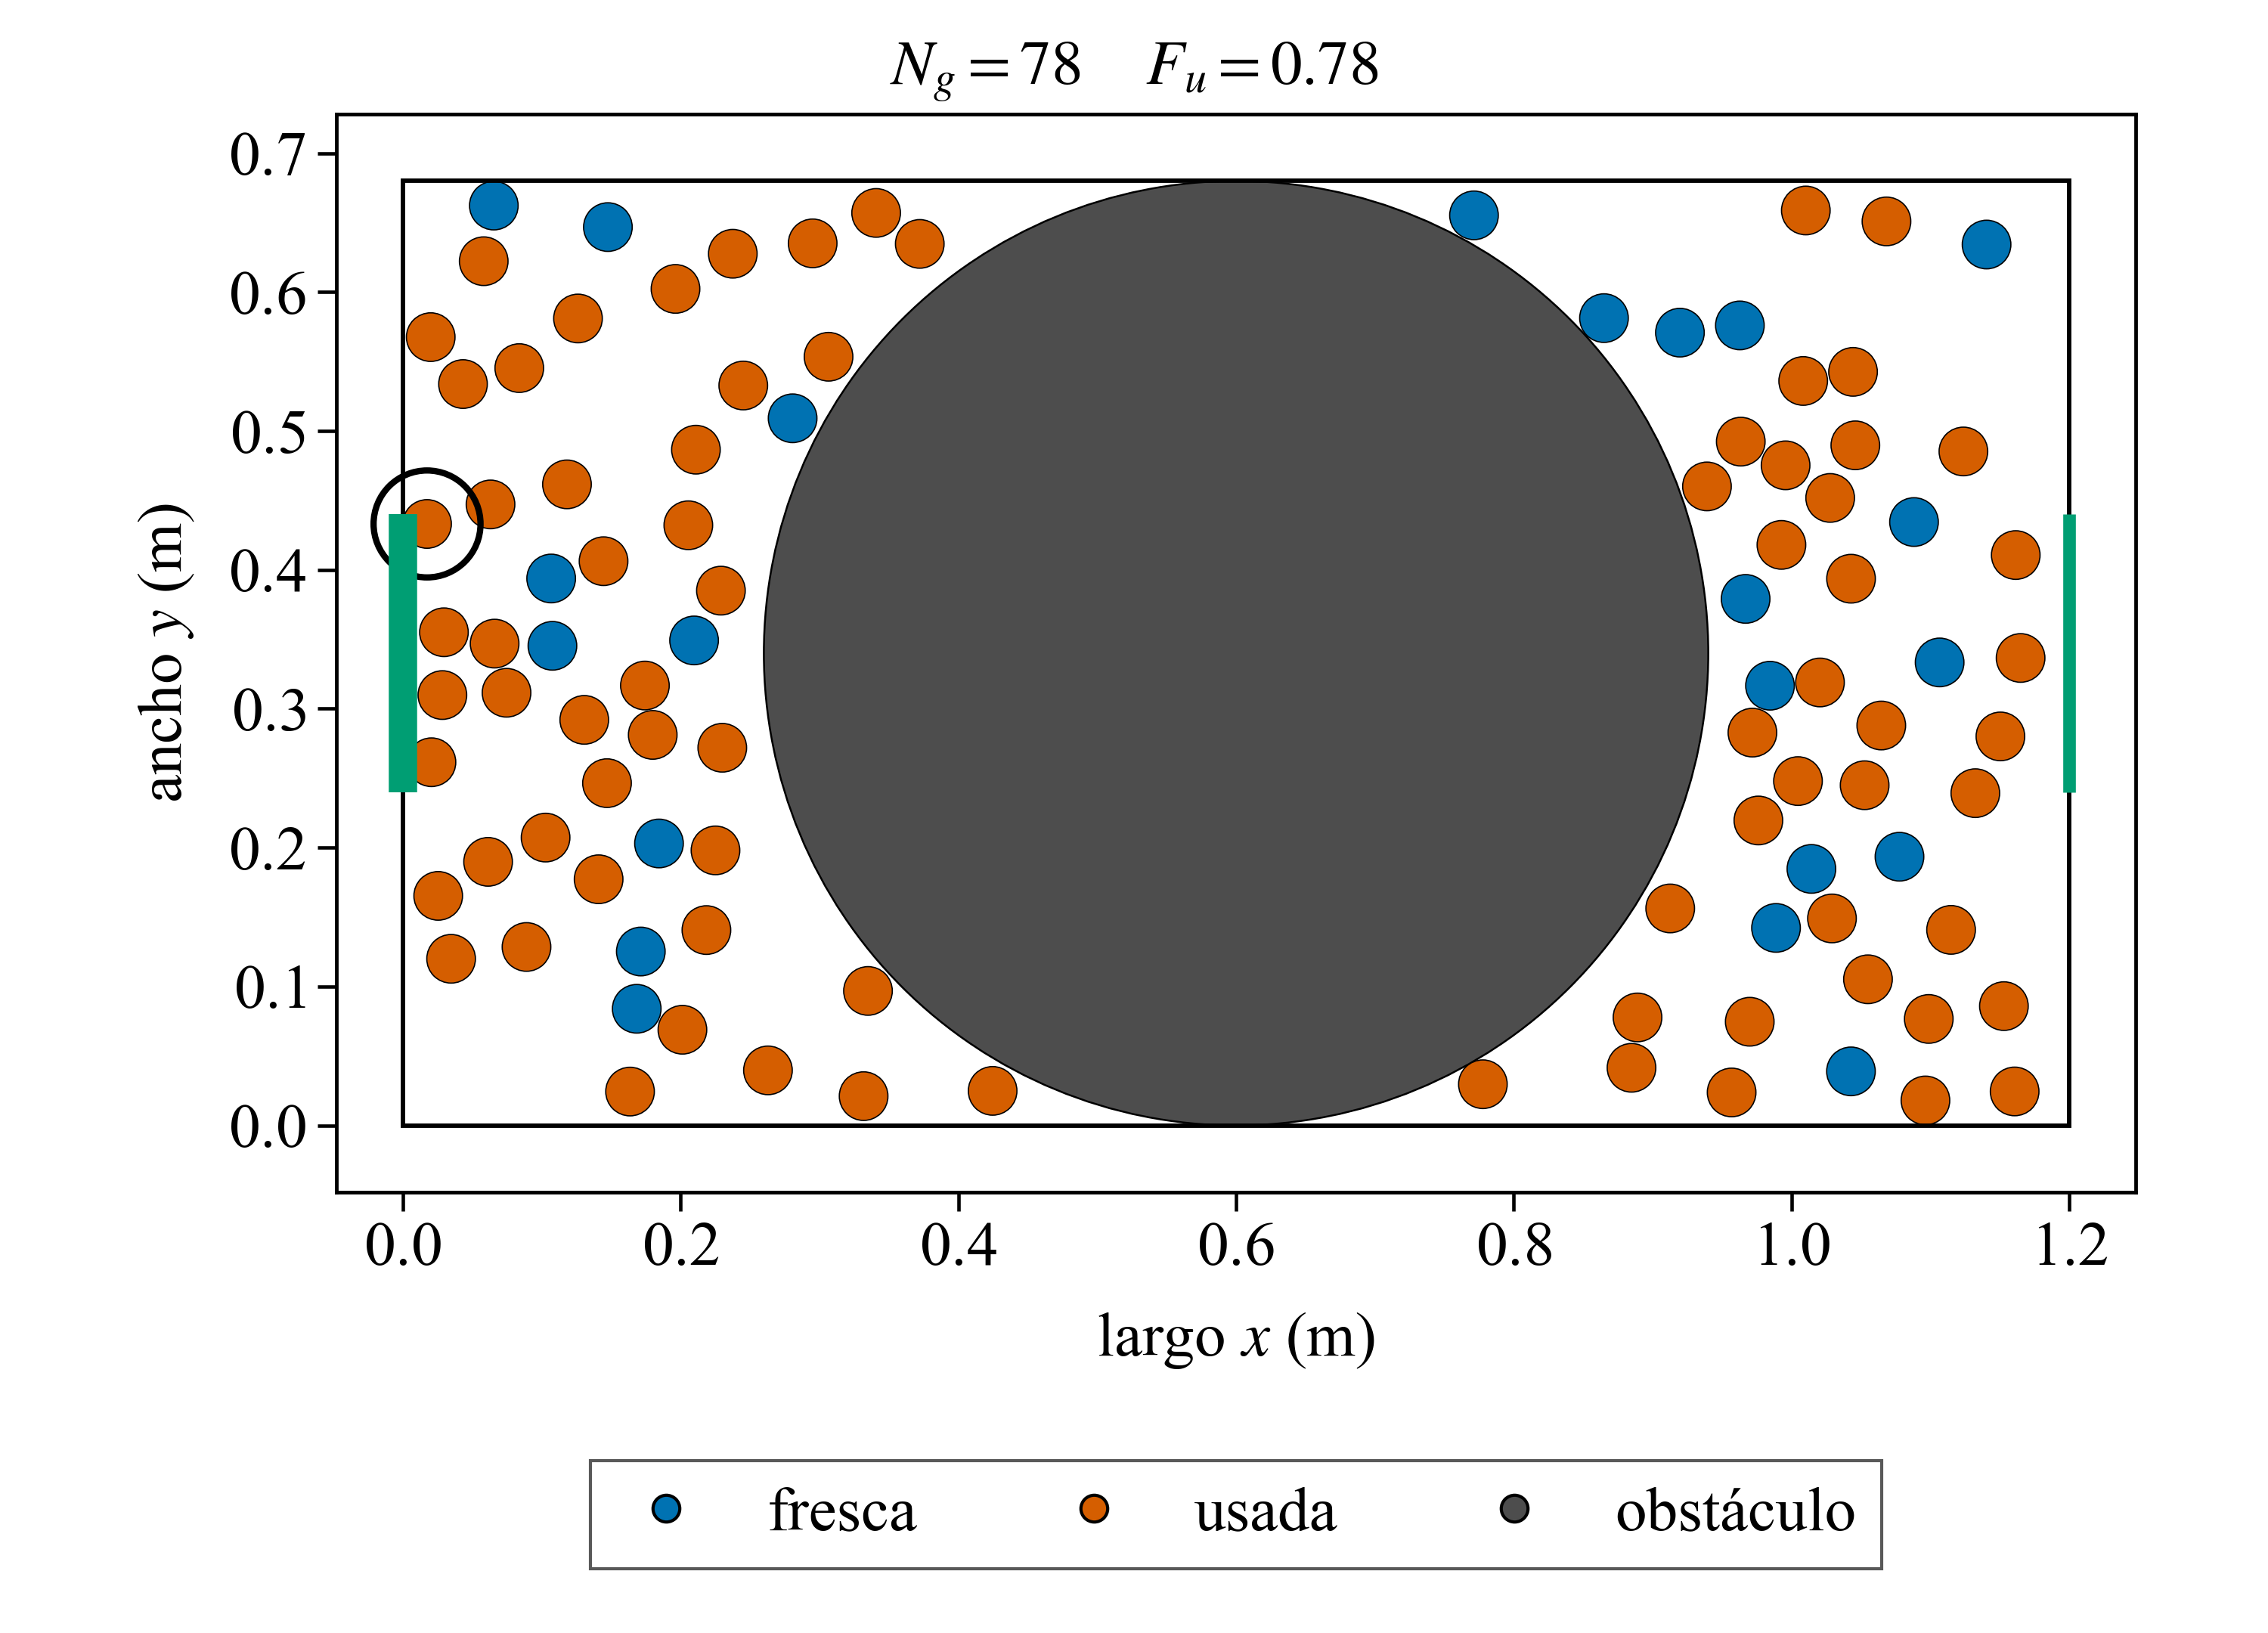
\includegraphics[width=\linewidth,height=0.88\textheight,keepaspectratio]{disco_r034.png}}{VPlayer.swf}
\end{frame}
\else 
    \begin{frame}{Evolución temporal}
          \begin{figure}
              \centering
          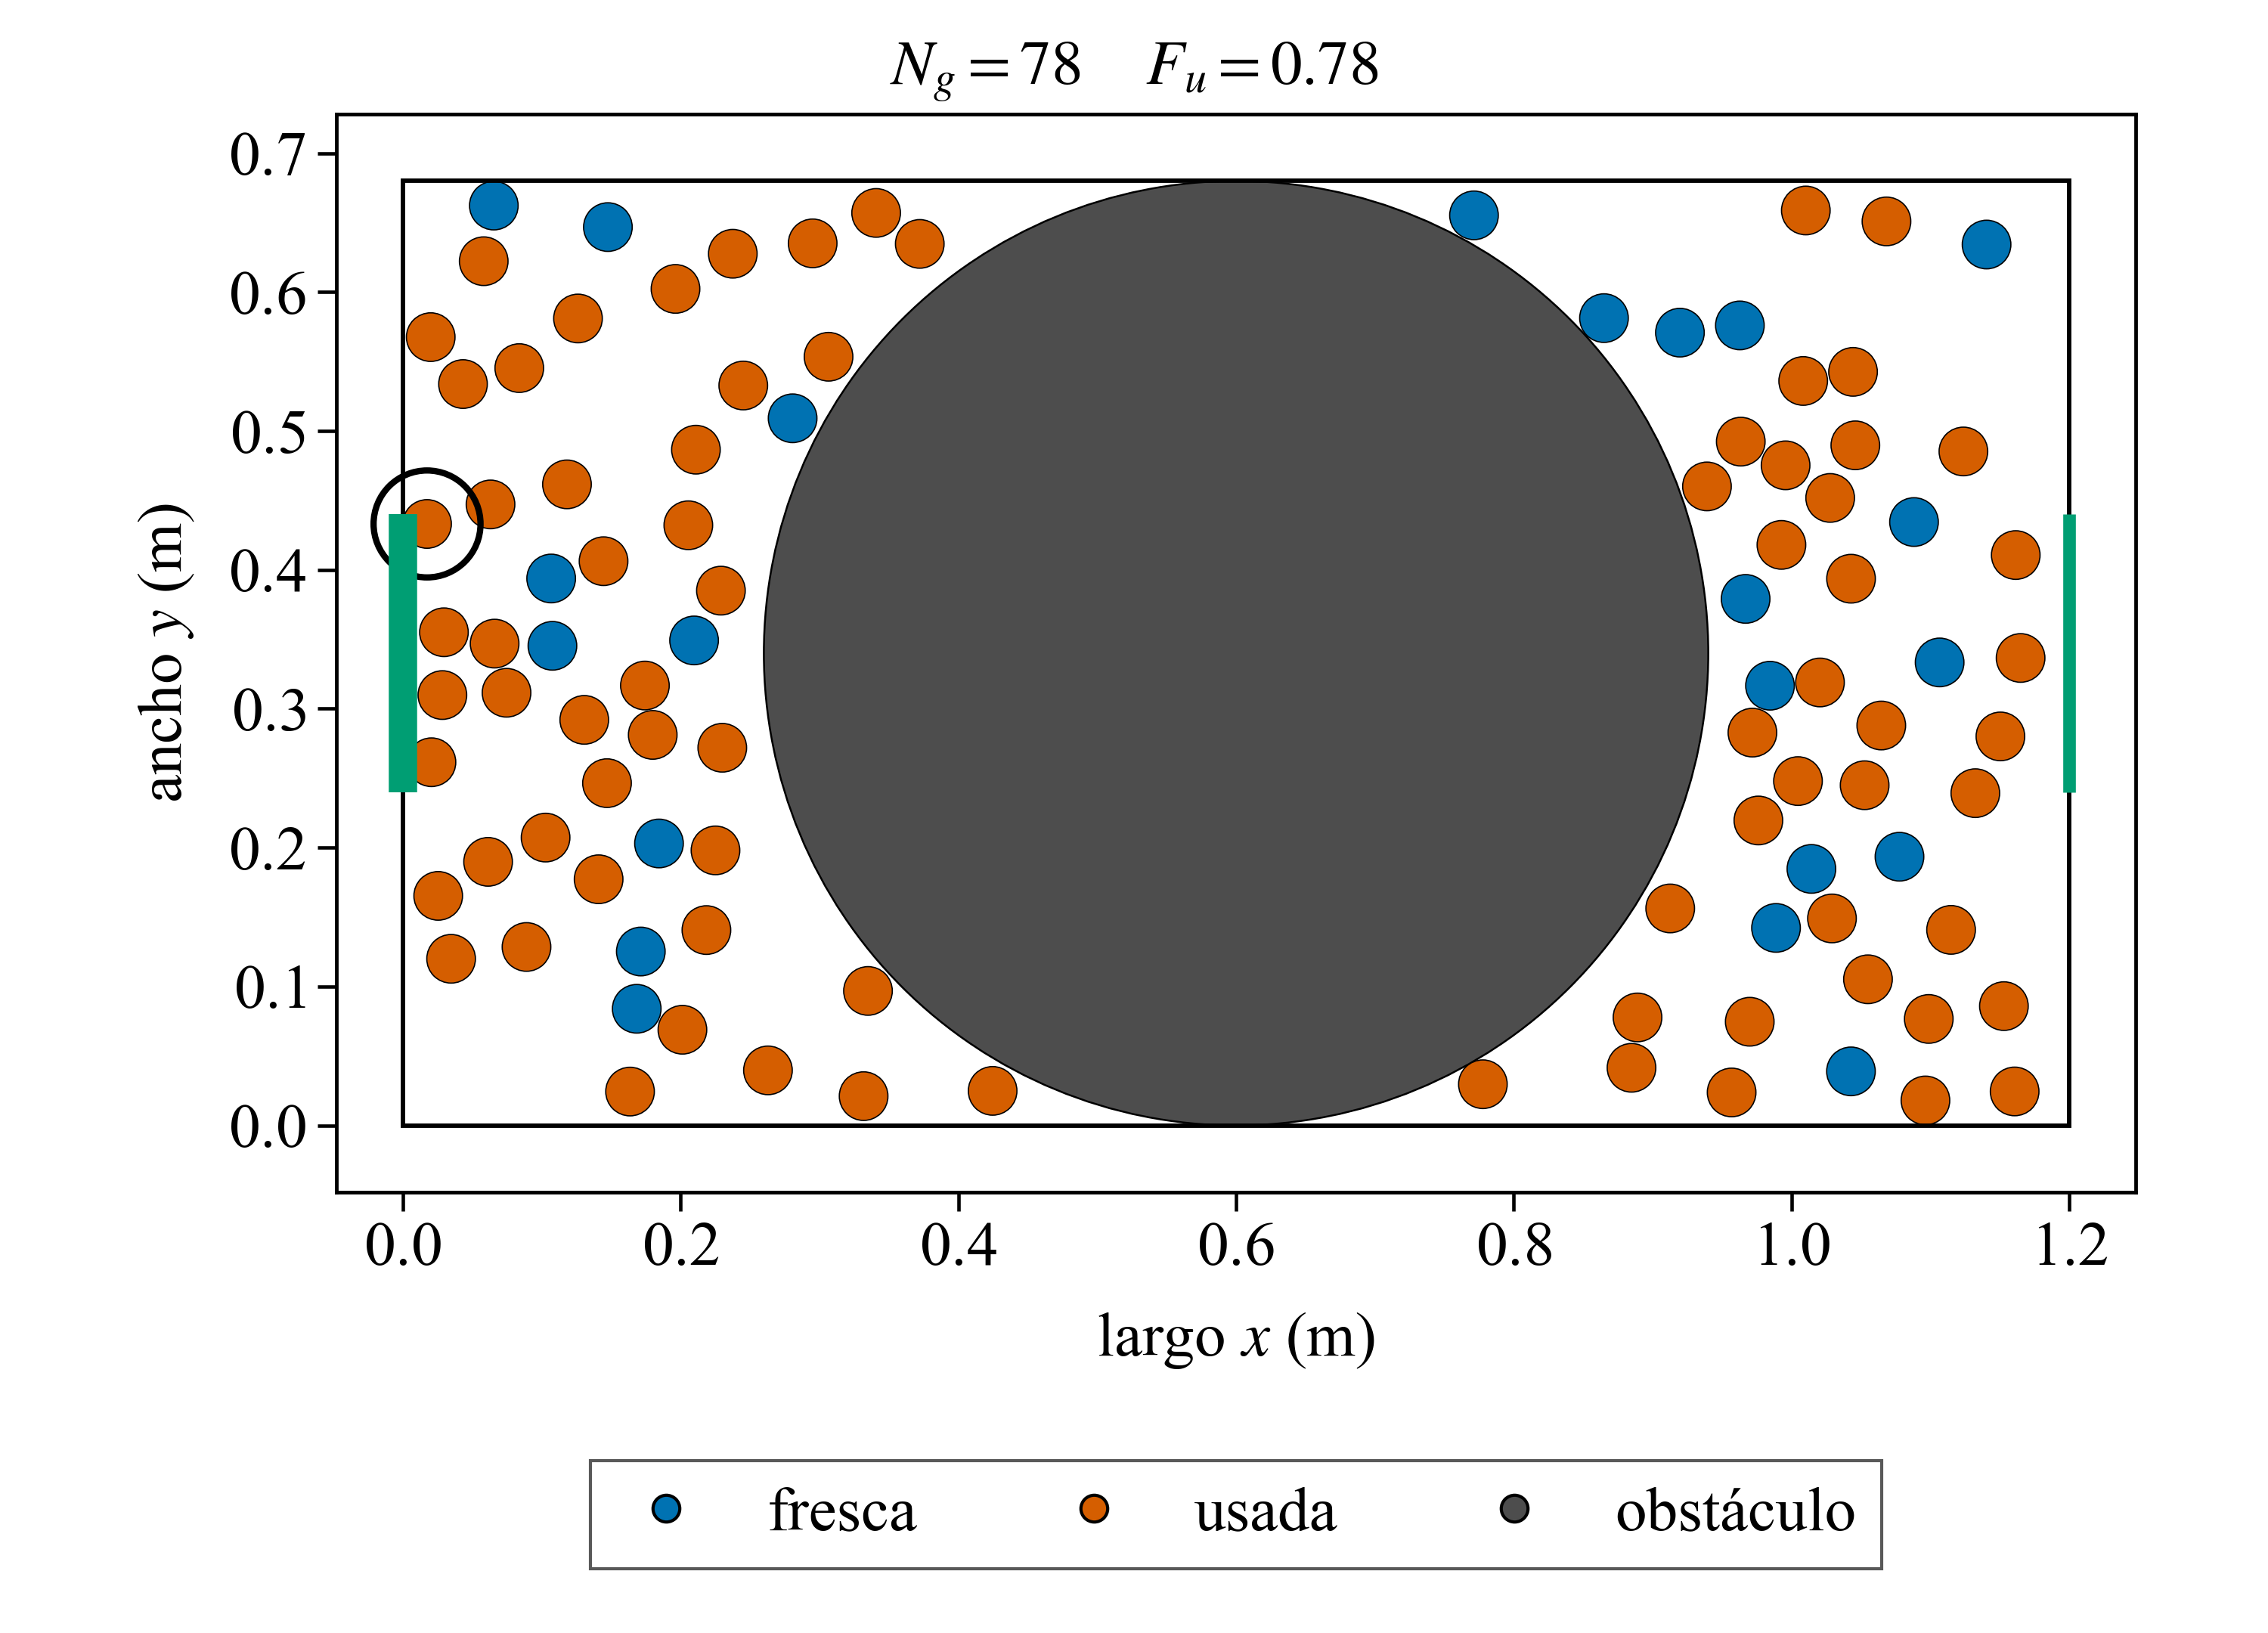
\includegraphics[width=\linewidth,height=0.78\textheight,keepaspectratio]{disco_r034.png}
                \caption*{\url{https://youtu.be/NNNVMJjTYGE?si=EVOp4JaLgAom3JTu}}        
            \end{figure}
    \end{frame}
    
\fi

\begin{frame}{Evolución de la fracción de partículas usadas}
  \centering
  \figura{fu_disco.png}
\end{frame}

\begin{frame}{$\langle t_{90}\rangle$ en función del radio}
  \begin{cols}
    \begin{column}{0.62\textwidth}
      \figura{disco_radio.png}
    \end{column}
    \begin{column}{0.34\textwidth}
      \begin{parametros}
        \item Centro fijo en $(0.60,\ 0.34)\,\mathrm{m}$
        \item $R$ de $0.06\,\mathrm{m}$ a $0.34\,\mathrm{m}$
      \end{parametros}
    \end{column}
  \end{cols}
\end{frame}

\begin{frame}{Pared de una columna}
  \begin{cols}
    \begin{column}{0.62\textwidth}
      \figura{pared_1.png}
    \end{column}
    \begin{column}{0.34\textwidth}
      \begin{parametros}
        \item 1 columna
        \item $R = 0.035\,\mathrm{m}$
        \item Centro $x = 0.60\,\mathrm{m}$
      \end{parametros}
      \begin{resultado}
        \item $\langle t_{90}\rangle = 21.50 \pm 1.86\,\mathrm{s}$
      \end{resultado}
    \end{column}
  \end{cols}
\end{frame}

\begin{frame}{$\langle t_{90}\rangle$ en función de las columnas, $R = 0.035\,\mathrm{m}$}
  \begin{cols}
    \begin{column}{0.62\textwidth}
      \figura{pared_cols_grandes.png}
    \end{column}
    \begin{column}{0.34\textwidth}
      \begin{parametros}
        \item $R = 0.035\,\mathrm{m}$
        \item Centro $x = 0.60\,\mathrm{m}$
      \end{parametros}
    \end{column}
  \end{cols}
\end{frame}

\begin{frame}{Pared de 9 columnas}
  \begin{cols}
    \begin{column}{0.62\textwidth}
      \figura{pared_9.png}
    \end{column}
    \begin{column}{0.34\textwidth}
      \begin{parametros}
        \item 9 columnas
        \item Ancho $= W$
        \item Centro $x = 0.60\,\mathrm{m}$
      \end{parametros}
      \begin{resultado}
        \item $\langle t_{90}\rangle = 14.21 \pm 1.41\,\mathrm{s}$
      \end{resultado}
    \end{column}
  \end{cols}
\end{frame}

\begin{frame}{Configuración de menor $\langle t_{90}\rangle$}
  \begin{cols}
    \begin{column}{0.62\textwidth}
      \figura{pared_18.png}
    \end{column}
    \begin{column}{0.34\textwidth}
      \begin{parametros}
        \item 18 columnas
        \item Ancho $0.644\,\mathrm{m}$
        \item $R = r$
        \item Centro $x = 0.60\,\mathrm{m}$
      \end{parametros}
      \begin{resultado}
        \item $\langle t_{90}\rangle = 13.67 \pm 1.31\,\mathrm{s}$
      \end{resultado}
    \end{column}
  \end{cols}
\end{frame}

\ifshowvideo
  \begin{frame}{Evolución temporal}
  \centering
  \includemedia[
    width=\linewidth,
    height=0.88\textheight,
    keepaspectratio,
    activate=pageopen,
    addresource=animations/pared_18.mp4,
    flashvars={
      source=animations/pared_18.mp4
      &autoPlay=true
      &loop=true
    }
  ]{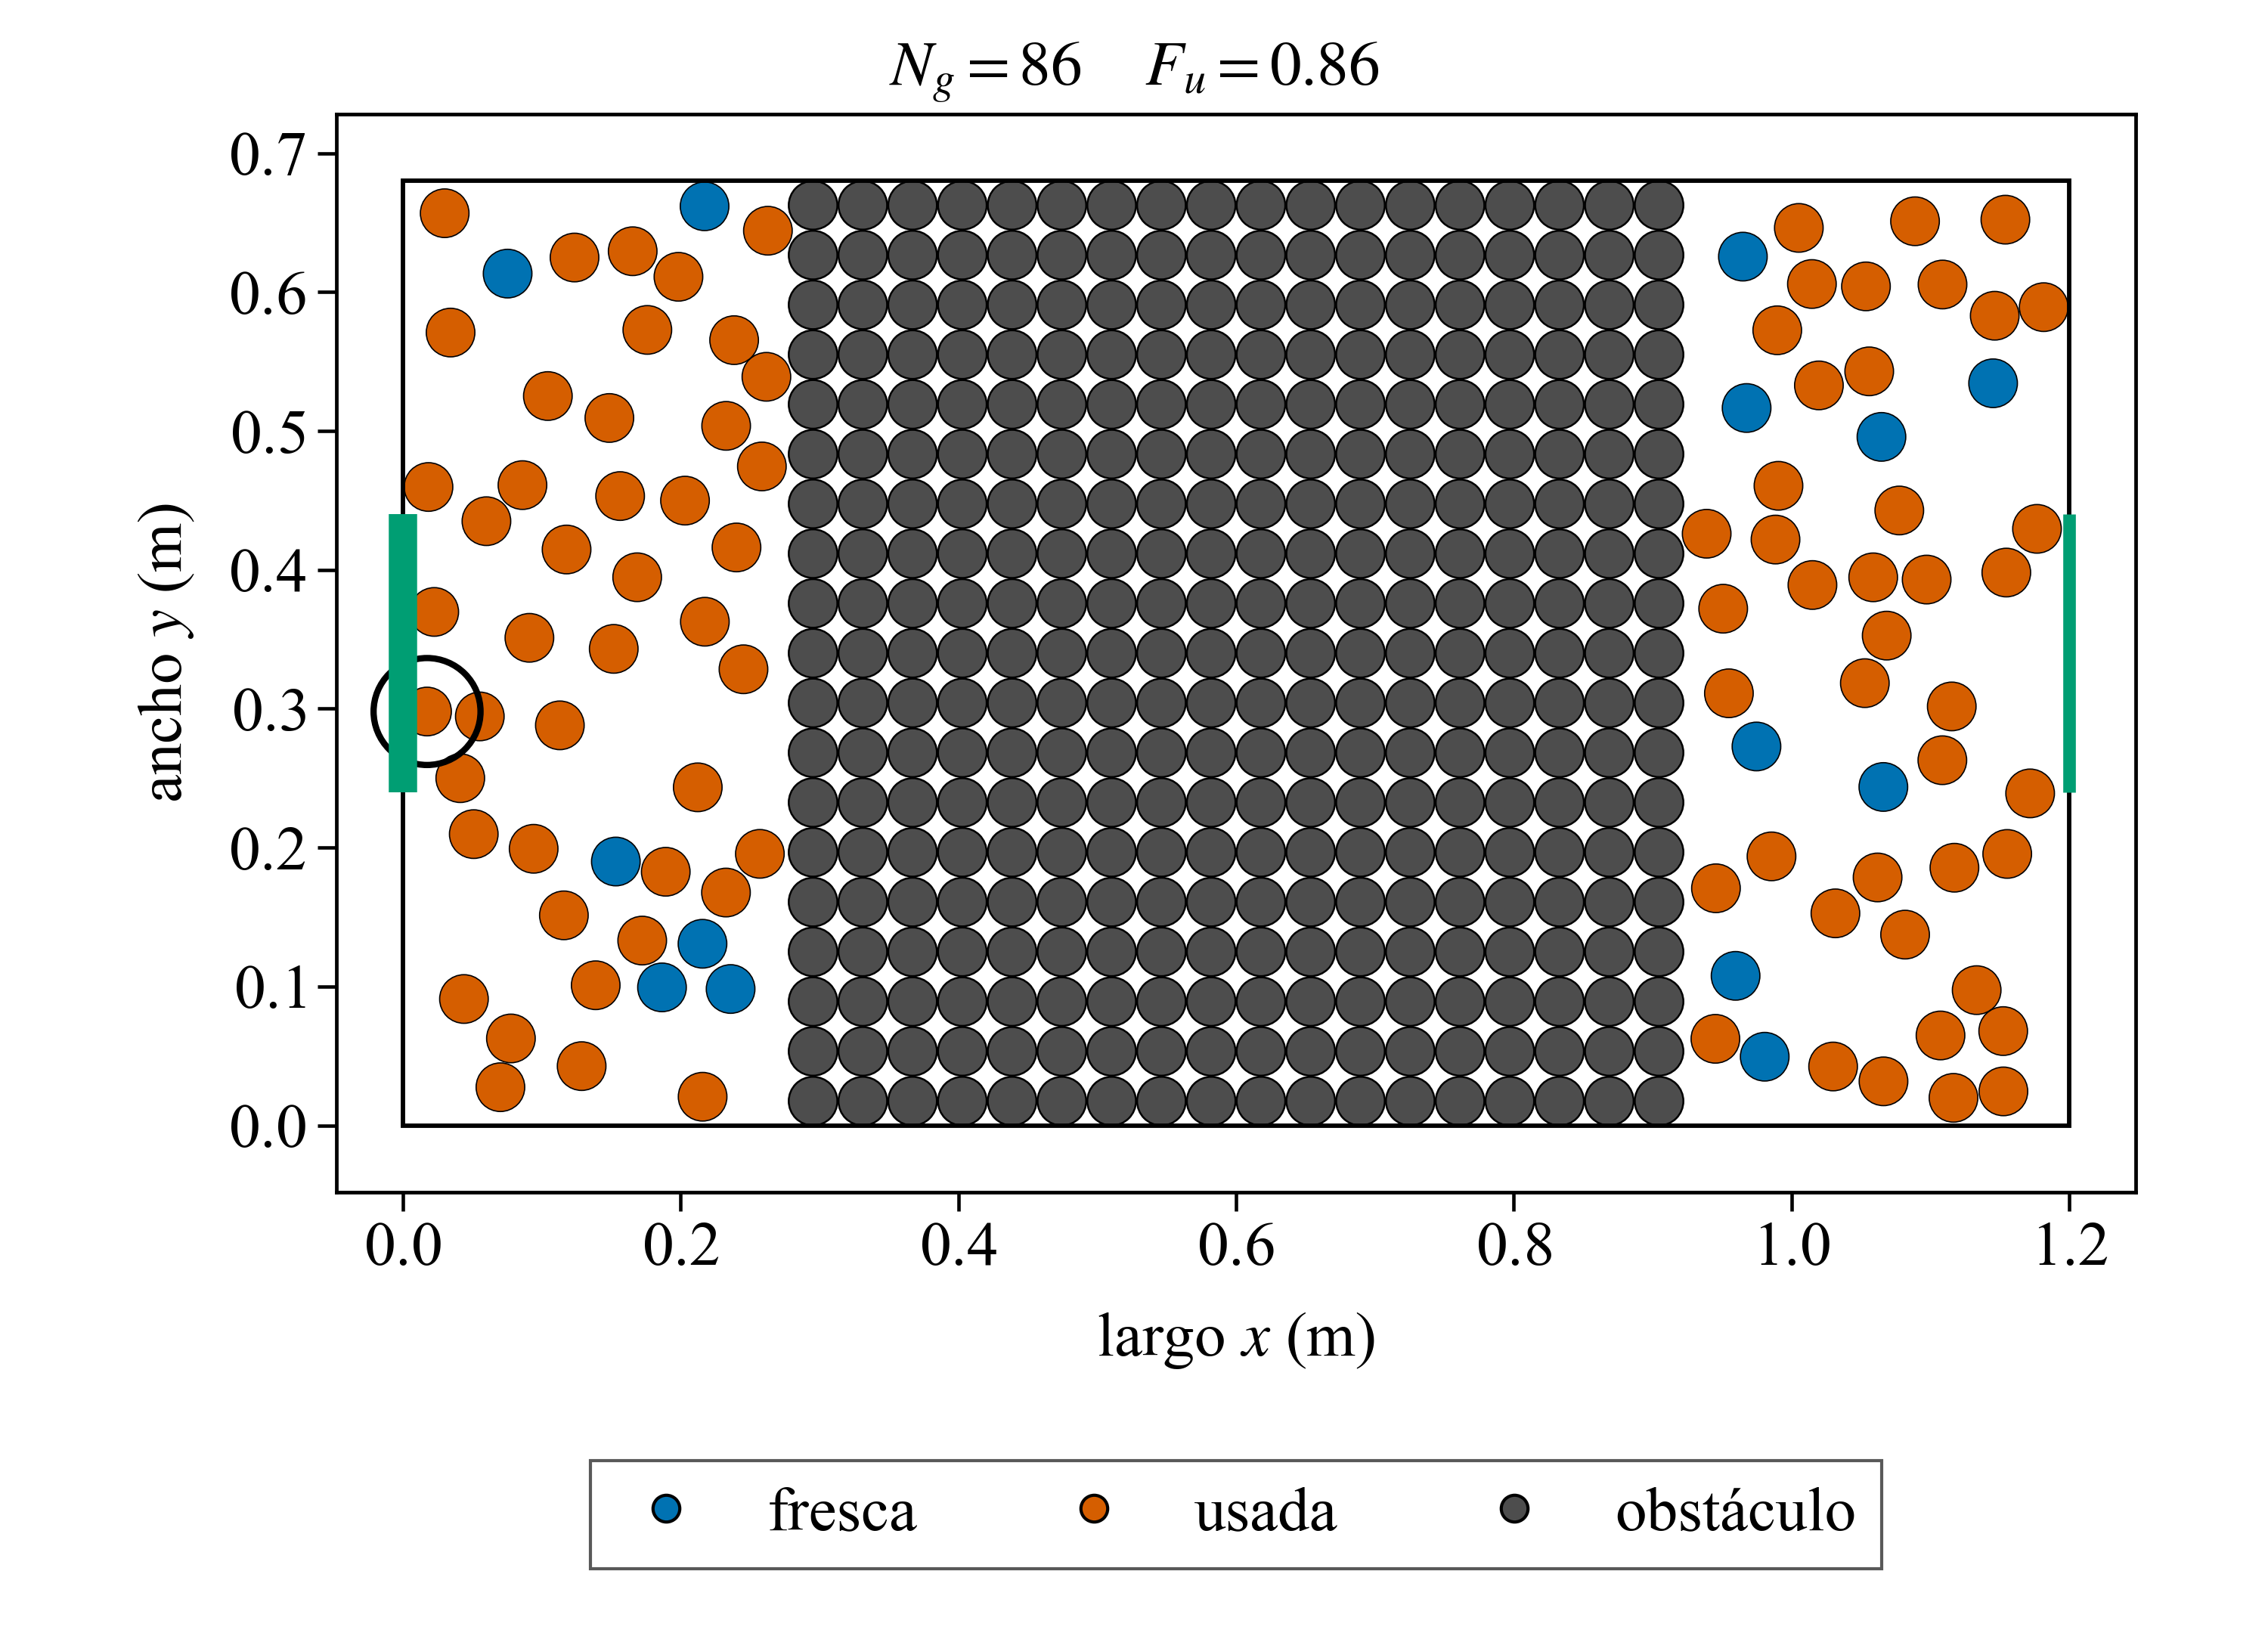
\includegraphics[width=\linewidth,height=0.88\textheight,keepaspectratio]{pared_18_anim.png}}{VPlayer.swf}
\end{frame}
\else 
    \begin{frame}{Evolución temporal}
          \begin{figure}
              \centering
          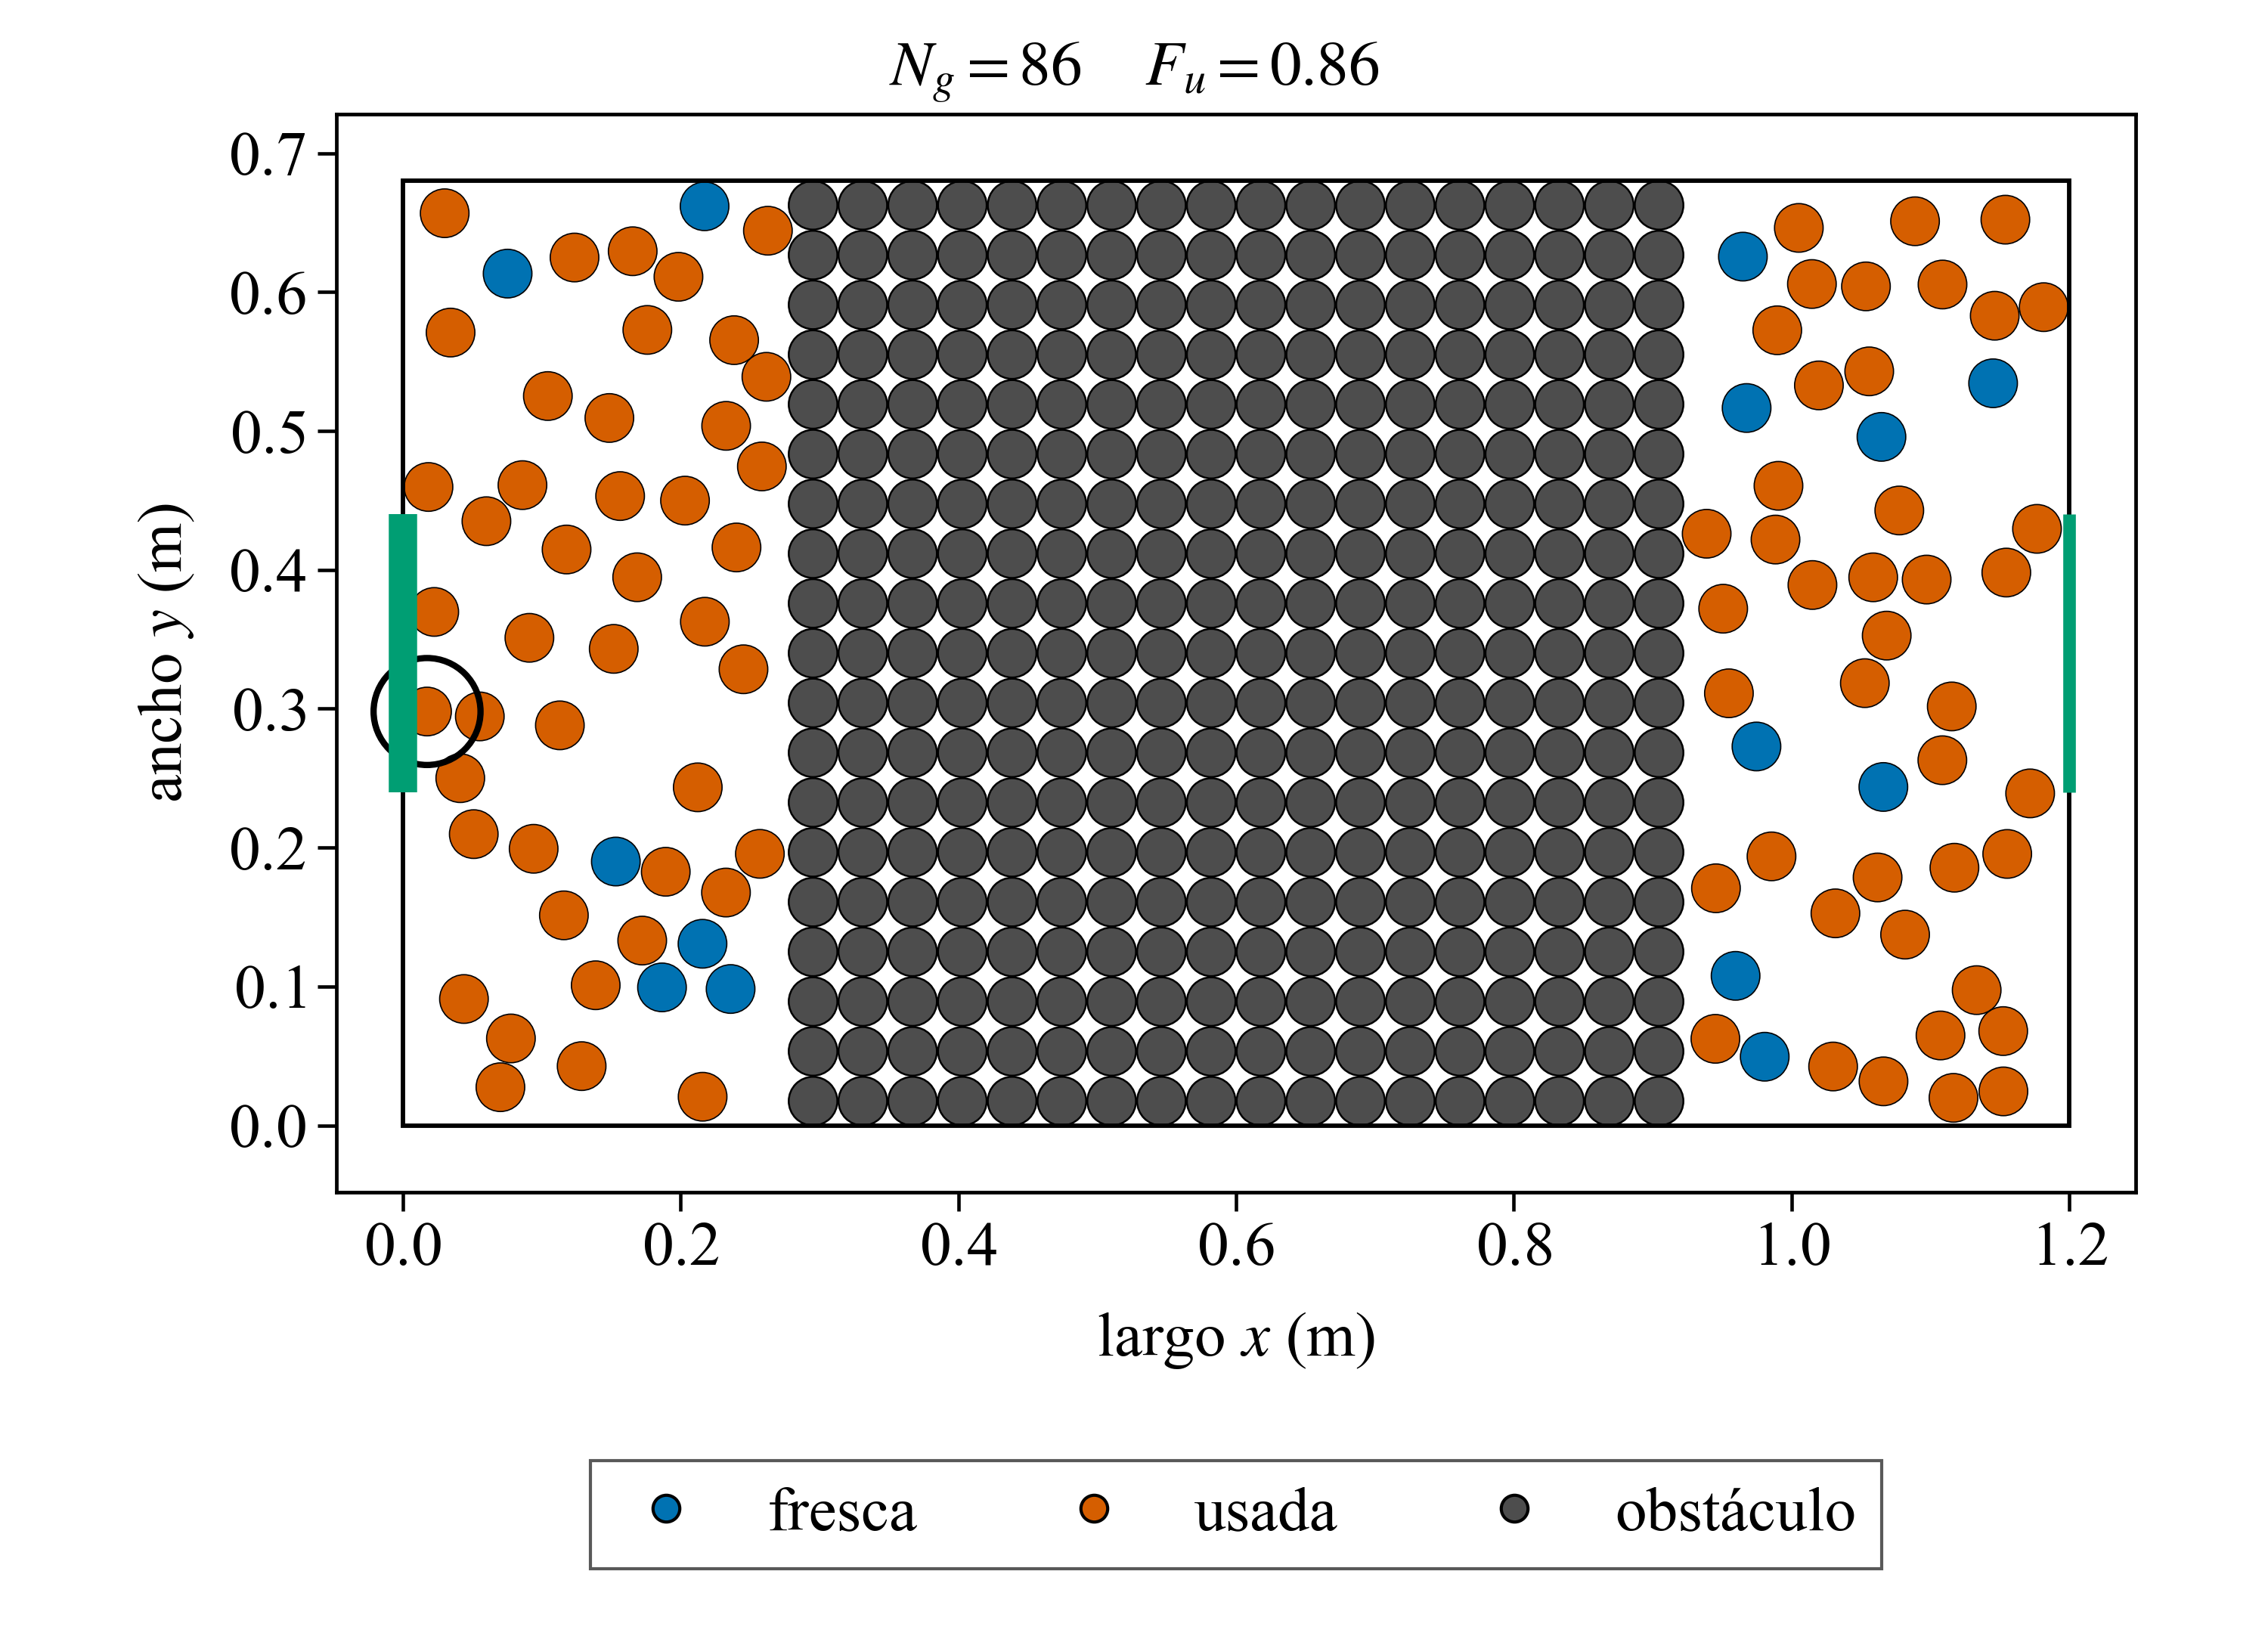
\includegraphics[width=\linewidth,height=0.78\textheight,keepaspectratio]{pared_18_anim.png}
                \caption*{\url{https://youtu.be/g3FZ9KBazS8?si=x4ou6pS7r4zBt_vN}}        
            \end{figure}
    \end{frame}
    
\fi

\begin{frame}{Evolución de la fracción de partículas usadas}
  \centering
  \figura{fu_ganador.png}
\end{frame}

\begin{frame}{$\langle t_{90}\rangle$ en función de las columnas, $R = r$}
  \begin{cols}
    \begin{column}{0.62\textwidth}
      \figura{pared_columnas.png}
    \end{column}
    \begin{column}{0.34\textwidth}
      \begin{parametros}
        \item $R = r$
        \item Centro $x = 0.60\,\mathrm{m}$
      \end{parametros}
    \end{column}
  \end{cols}
\end{frame}

\subsection{DCM y coeficiente de difusión}


\begin{frame}{Desplazamiento cuadrático medio}
  \begin{cols}
    \begin{column}{0.62\textwidth}
      \figura{dcm_vacia.png}
    \end{column}
    \begin{column}{0.34\textwidth}
      \begin{parametros}
        \item Mesa vacía, $N = 100$, $t_f = 30\,\mathrm{s}$
        \item $t_e$ estacionario según configuración obstáculos
      \end{parametros}
      \begin{resultado}
        \item $D = \DcmDvacia\,\mathrm{m}^{2}/\mathrm{s}$
      \end{resultado}
      {\scriptsize DCM una realización. $D$: promedio ajustes de $10$ realizaciones.}
    \end{column}
  \end{cols}
\end{frame}

\begin{frame}{Ajuste de $\langle \Delta r^{2}\rangle = 4Dt + b$}
  \begin{cols}
    \begin{column}{0.62\textwidth}
      \figura{dcm_error.png}
    \end{column}
    \begin{column}{0.34\textwidth}
      \begin{parametros}
        \item Puntos en $[0, t_e]$ de una realización
        \item Semilla 401
      \end{parametros}
      \begin{resultado}
        \item $D^{*} = \DcmDejemplo\,\mathrm{m}^{2}/\mathrm{s}$
      \end{resultado}
    \end{column}
  \end{cols}
\end{frame}

\begin{frame}{Desplazamiento cuadrático medio según la configuración}
    \centering   
      \figura{dcm_configs.png}
\end{frame}

\begin{frame}{$D$ y $\langle t_{90}\rangle$}
  \centering\small
  \renewcommand{\arraystretch}{1.35}
  % Generado por python/dcm_report.py (docs/results/1.3/cortes.txt). No editar a mano.
\begin{tabular}{lccccc}
  \hline
  configuración & divide la mesa & $t_m$ (s) & $D$ (m$^{2}$/s) & meseta (m$^{2}$) & $\langle t_{90}\rangle$ (s) \\
  \hline
  mesa vacía & no & $6$ & $0.0098 \pm 0.0014$ & $0.284 \pm 0.015$ & $24 \pm 3$ \\
  disco, $R = 0.22\,\mathrm{m}$ & no & $20$ & $0.0044 \pm 0.0007$ & $0.41 \pm 0.04$ & $20 \pm 3$ \\
  disco, $R = 0.34\,\mathrm{m}$ & sí & $10$ & $0.0019 \pm 0.0002$ & $0.105 \pm 0.005$ & $17.0 \pm 2.0$ \\
  pared, 9 columnas & sí & $4$ & $0.0035 \pm 0.0005$ & $0.075 \pm 0.003$ & $14.2 \pm 1.4$ \\
  pared, 18 columnas & sí & $9$ & $0.0020 \pm 0.0003$ & $0.079 \pm 0.006$ & $13.7 \pm 1.3$ \\
  \hline
\end{tabular}

  \par\vspace{8pt}
\end{frame}


\begin{frame}{$\langle t_{90}\rangle$ y $D$ según las columnas}
  \begin{cols}
    \begin{column}{0.62\textwidth}
      \figura{t90_d_vs_columnas.png}
    \end{column}
    \begin{column}{0.34\textwidth}
      \begin{parametros}
        \item Pared $R = r$, centro $x = 0.60\,\mathrm{m}$
        \item Línea punteada: 18 columnas
      \end{parametros}
      \begin{resultado}
        \item Tendencia compartida hasta 18 columnas
        \item Luego del óptimo comportamiento diferente
      \end{resultado}
    \end{column}
  \end{cols}
\end{frame}

\begin{frame}{Conclusiones}
  \begin{itemize}\setlength{\itemsep}{14pt}
    \item Hasta $N \approx 300$ tiempo \textbf{crece} $O(N^{3})$.
    \item Separar mesa \textbf{en dos} \textbf{baja} $\langle t_{90}\rangle$ hasta óptimo 18 columnas $R=r$.
    \item $D$ disminuye con obstáculos.
    \item $\langle t_{90}\rangle$ y $D$ disminuyen juntos solo hasta óptimo.
  \end{itemize}
\end{frame}

\begin{frame}[plain,noframenumbering]
  \vfill\centering{\Huge\usebeamercolor[fg]{structure}Muchas gracias}\vfill
\end{frame}

% Respaldo para preguntas (no se presenta).
% Punto 1: docs/results/1.1/1.1_tiempo_de_ejecucion.md.
\begin{frame}[noframenumbering]{Apéndice: ajuste de la ley de potencia}
  \begin{cols}
    \begin{column}{0.55\textwidth}
      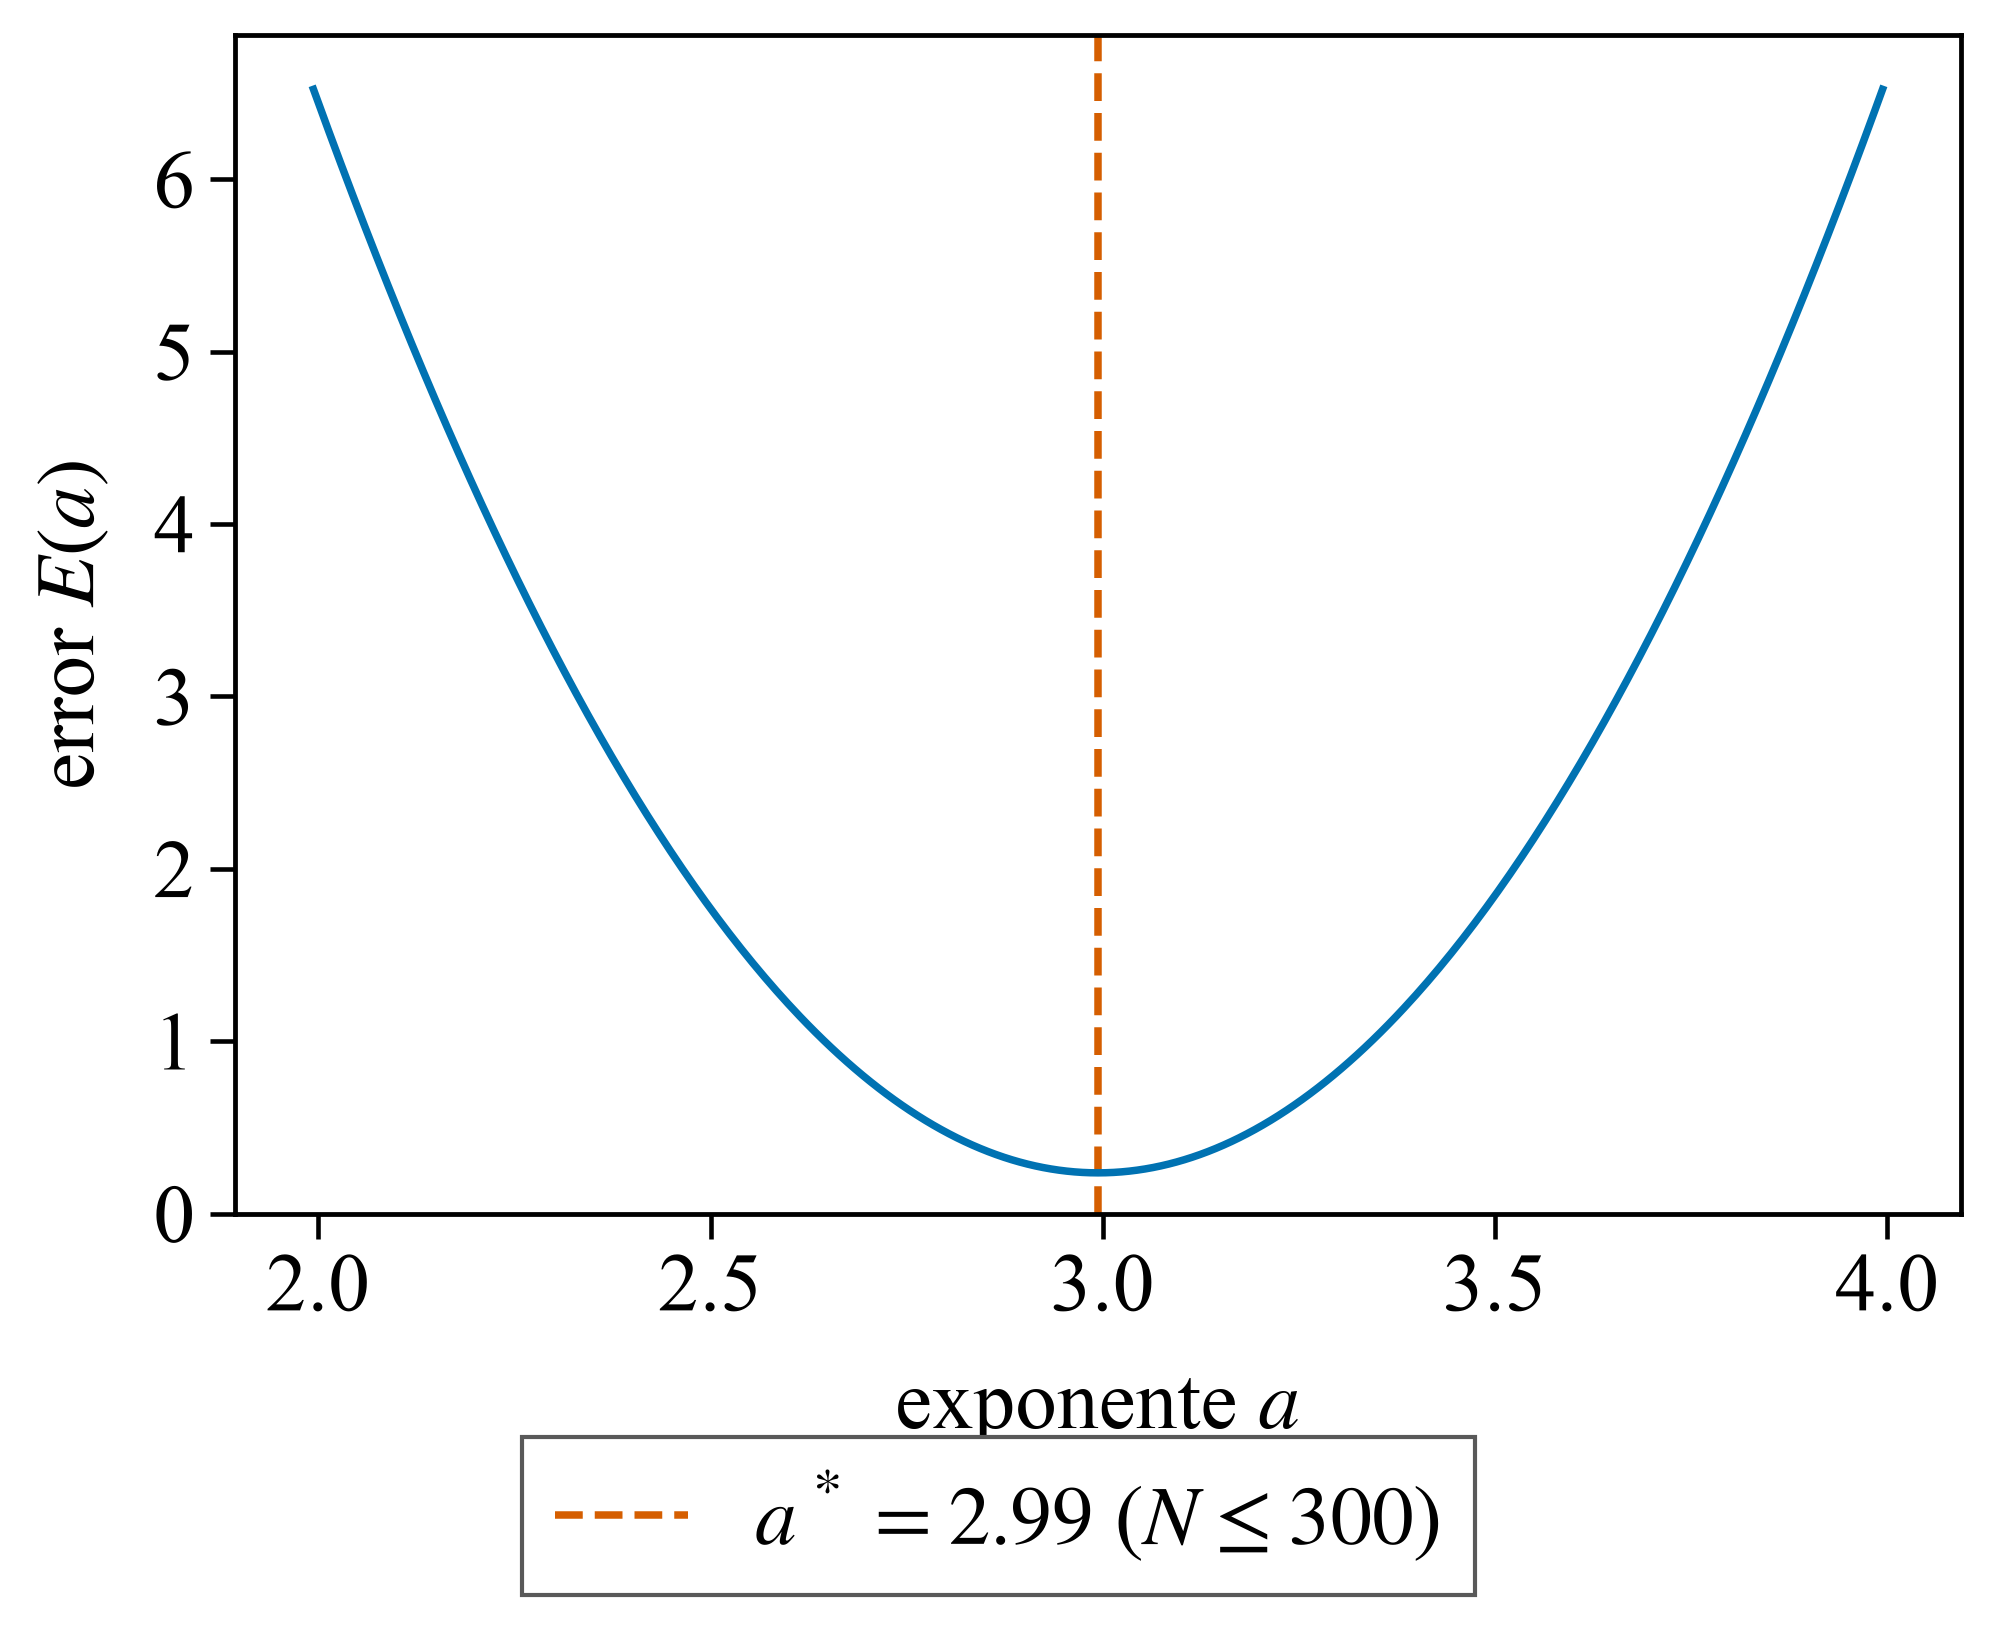
\includegraphics[width=\linewidth,height=0.78\textheight,keepaspectratio]{runtime_error.png}
    \end{column}
    \begin{column}{0.42\textwidth}
      \small
      Modelo $t = c\,N^{a}$. Con logaritmos:
      \[ \log t = \log c + a \log N \]
      Para cada $a$, el mejor $\log c$ y el error:
      \[ E(a) = \sum_{i=1}^{12}\left[\log t_i - \log c(a) - a\log N_i\right]^{2} \]
      $12$ puntos con $N \leq 300$, $t_i$ = promedio de $10$ realizaciones.
      \begin{resultado}
        \item Mínimo en $a = 2.99 \pm 0.06$
      \end{resultado}
    \end{column}
  \end{cols}
\end{frame}

\begin{frame}[noframenumbering]{Apéndice: por qué $N^{3}$}
  \begin{cols}
    \begin{column}{0.49\textwidth}
      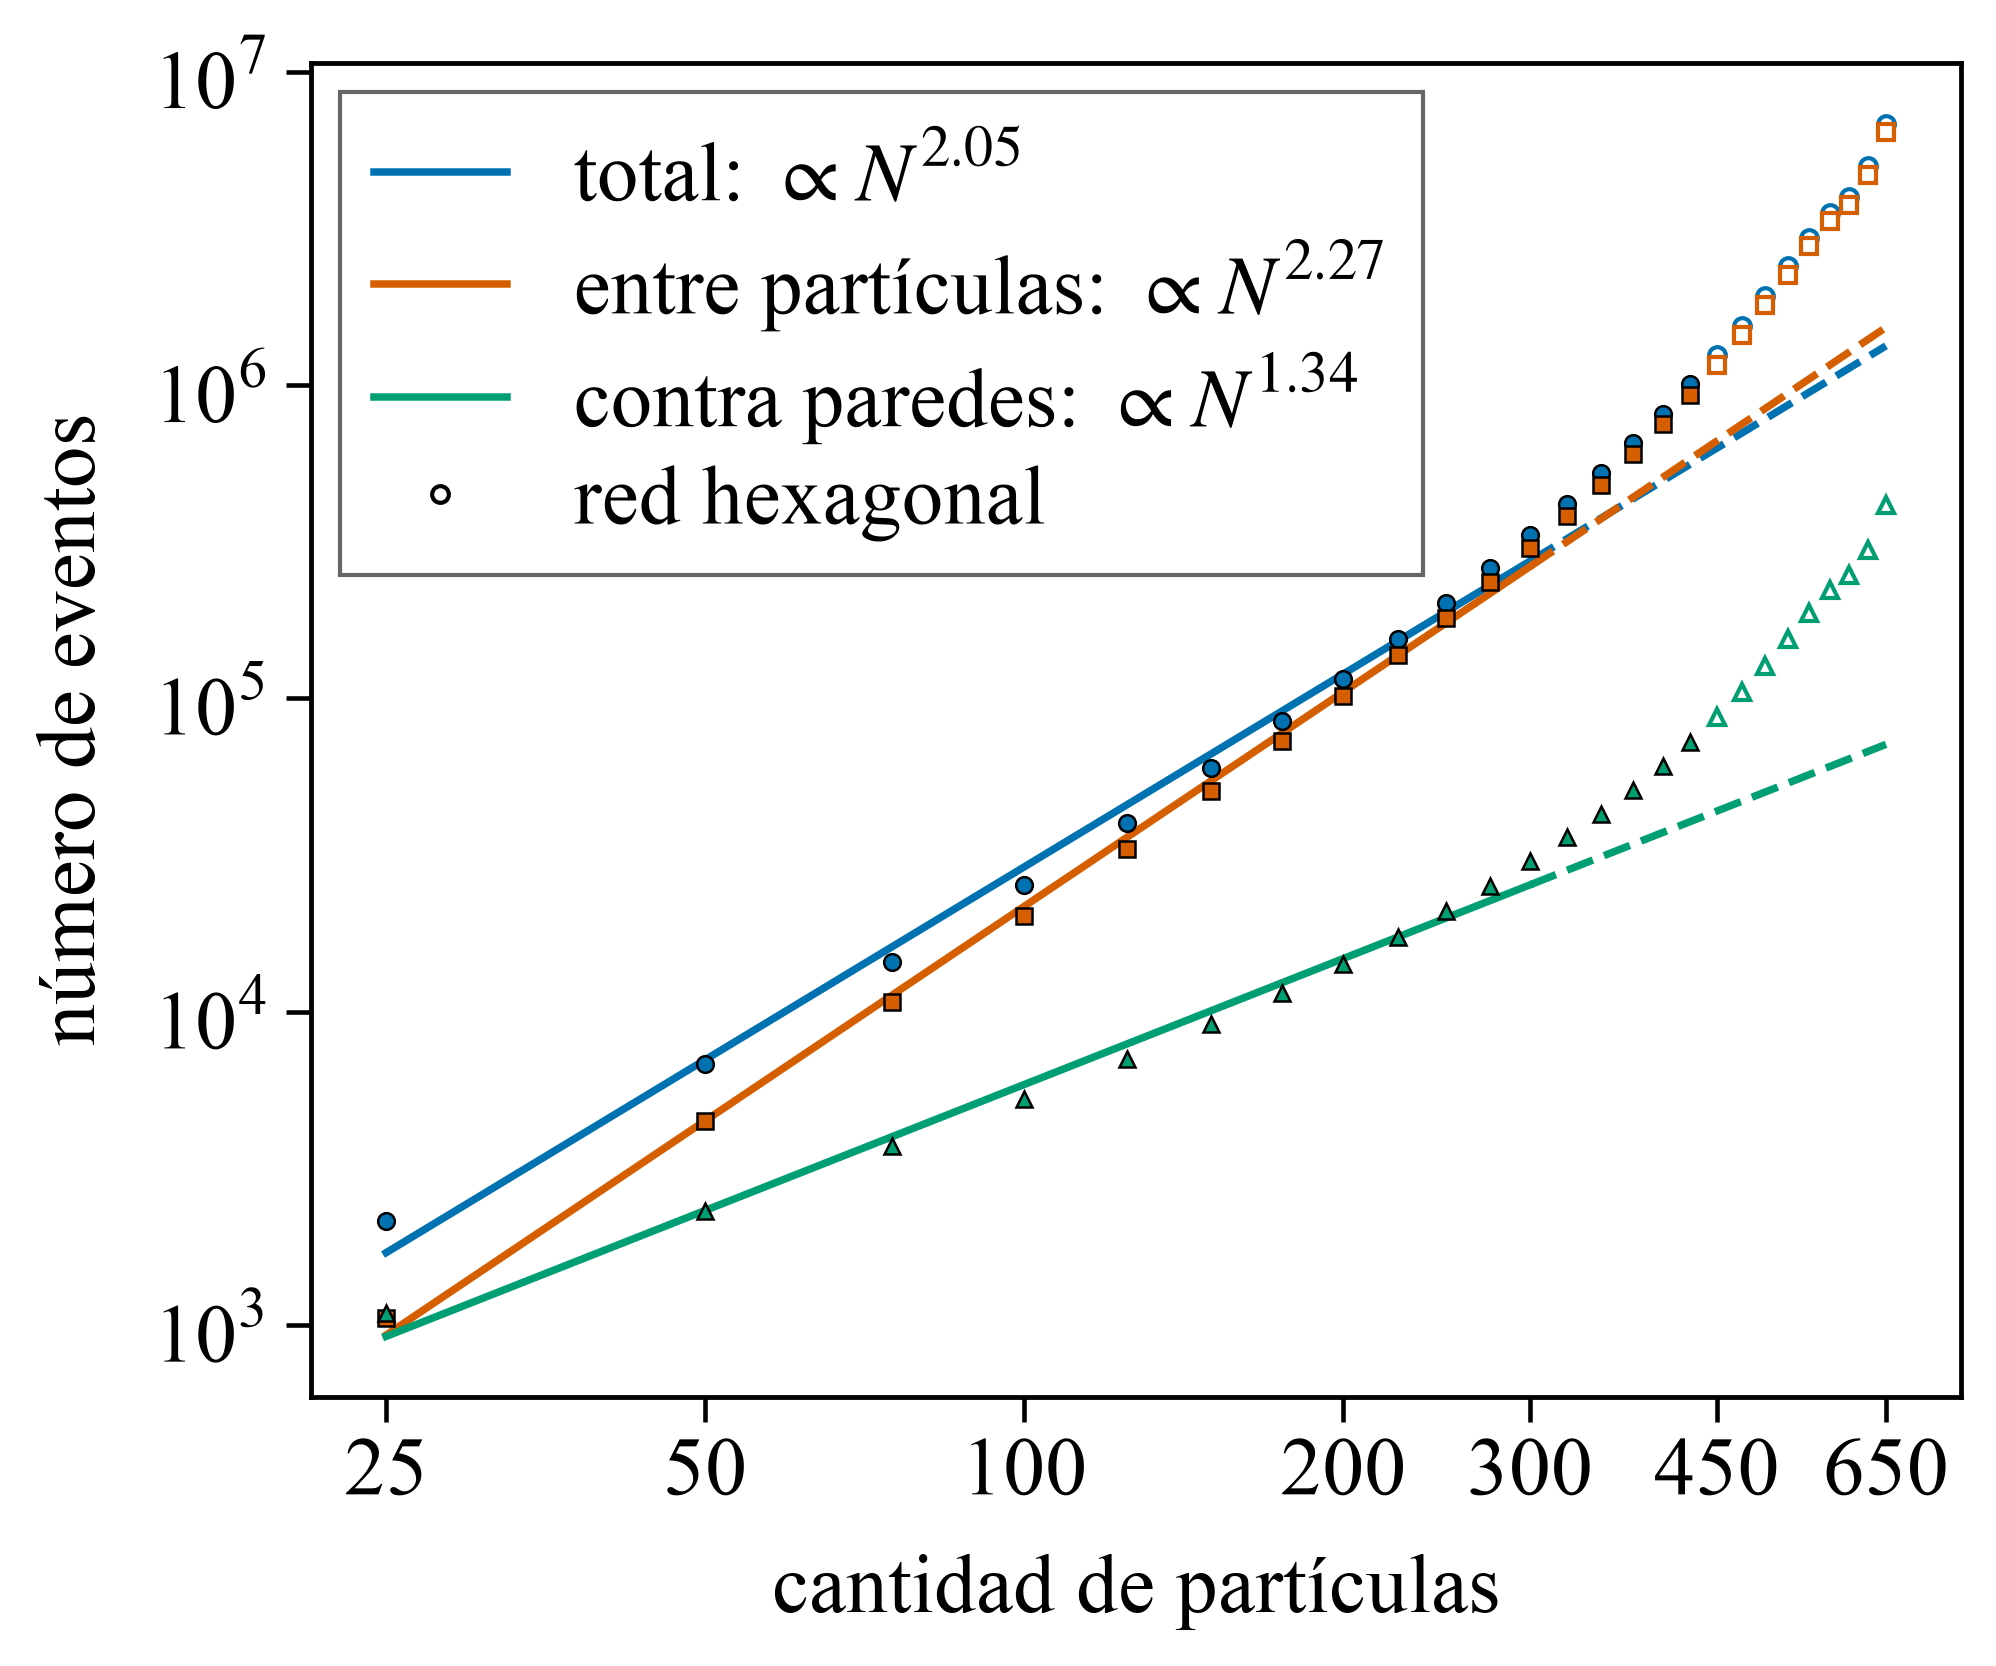
\includegraphics[width=\linewidth,height=0.6\textheight,keepaspectratio]{runtime_events_loglog.png}
    \end{column}
    \begin{column}{0.49\textwidth}
      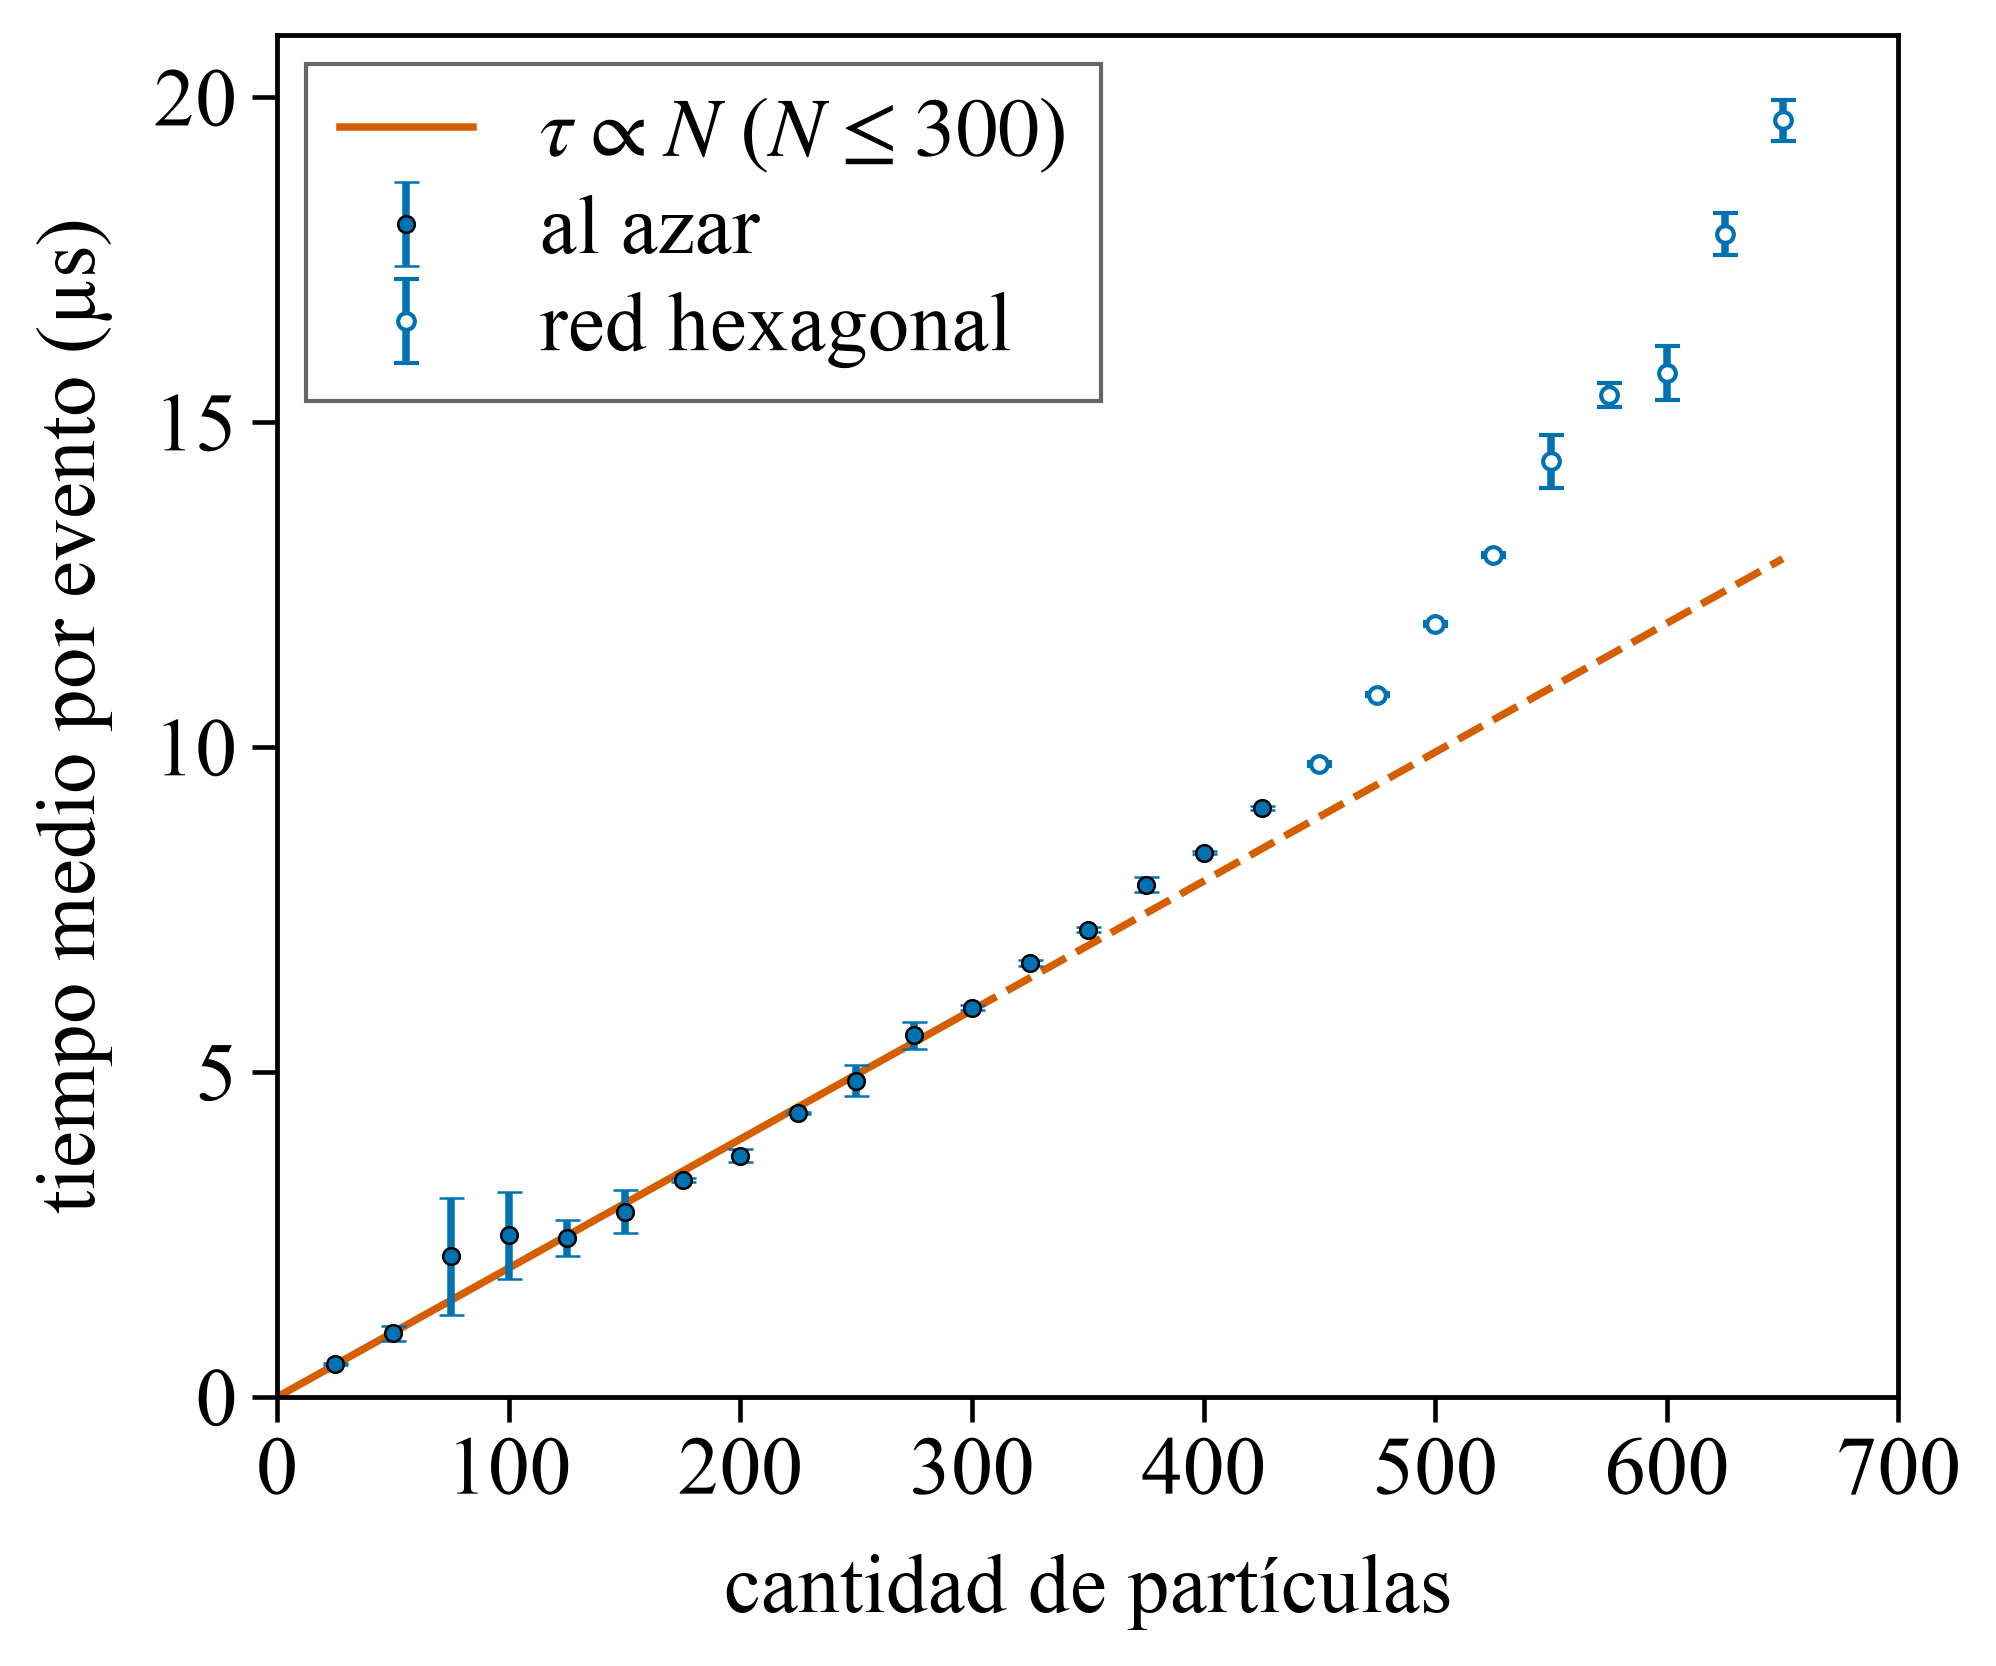
\includegraphics[width=\linewidth,height=0.6\textheight,keepaspectratio]{runtime_per_event.png}
    \end{column}
  \end{cols}
  \small
  \[ t = \underbrace{E(N)}_{\propto N^{2.05}} \cdot \underbrace{\tau(N)}_{\propto N^{0.95}} \propto N^{3.0} \]
  {\footnotesize $E$: eventos en $30\,\mathrm{s}$ (más partículas, y cada una choca más seguido).
  $\tau$: costo por evento; se avanzan las $N$ partículas y se recalculan los choques de la que chocó contra las otras $N$.}
\end{frame}

% Punto 3: figuras y tablas generadas por python/dcm_report.py y
% python/dcm_barrido.py a partir de cortes*.txt.
\begin{frame}[noframenumbering]{Apéndice: cálculo del DCM y de $D$}
  \small
  \begin{enumerate}\setlength{\itemsep}{6pt}
    \item Estado guardado cada $10$ eventos (y en cada gol), en su tiempo de evento.
    \item En cada cuadro, promedio sobre las $N = 100$ partículas (frescas y usadas):
          \[ \langle\Delta r^{2}\rangle(t) = \frac{1}{N}\sum_{i=1}^{N}\left|\vv{r}_i(t) - \vv{r}_i(0)\right|^{2} \]
    \item $t_e$: inicio del estacionario, elegido a ojo sobre la curva de $30\,\mathrm{s}$.
    \item Ajuste en $[0, t_e]$ (Teórica 0), con $b(D)$ el mejor $b$ para cada $D$:
          \[ E(D) = \sum_{i}\left[\langle\Delta r^{2}\rangle_i - 4Dt_i - b(D)\right]^{2}, \qquad D = \frac{\text{pendiente}}{4} \]
    \item Se repite en $10$ realizaciones: $\langle D\rangle \pm$ desvío estándar.
  \end{enumerate}
  {\footnotesize Se promedian escalares ($D$, $t_{90}$) entre realizaciones, no curvas: los tiempos de evento de dos corridas no coinciden.}
\end{frame}

\begin{frame}[noframenumbering]{Apéndice: elección de $t_e$ por configuración}
  \centering
  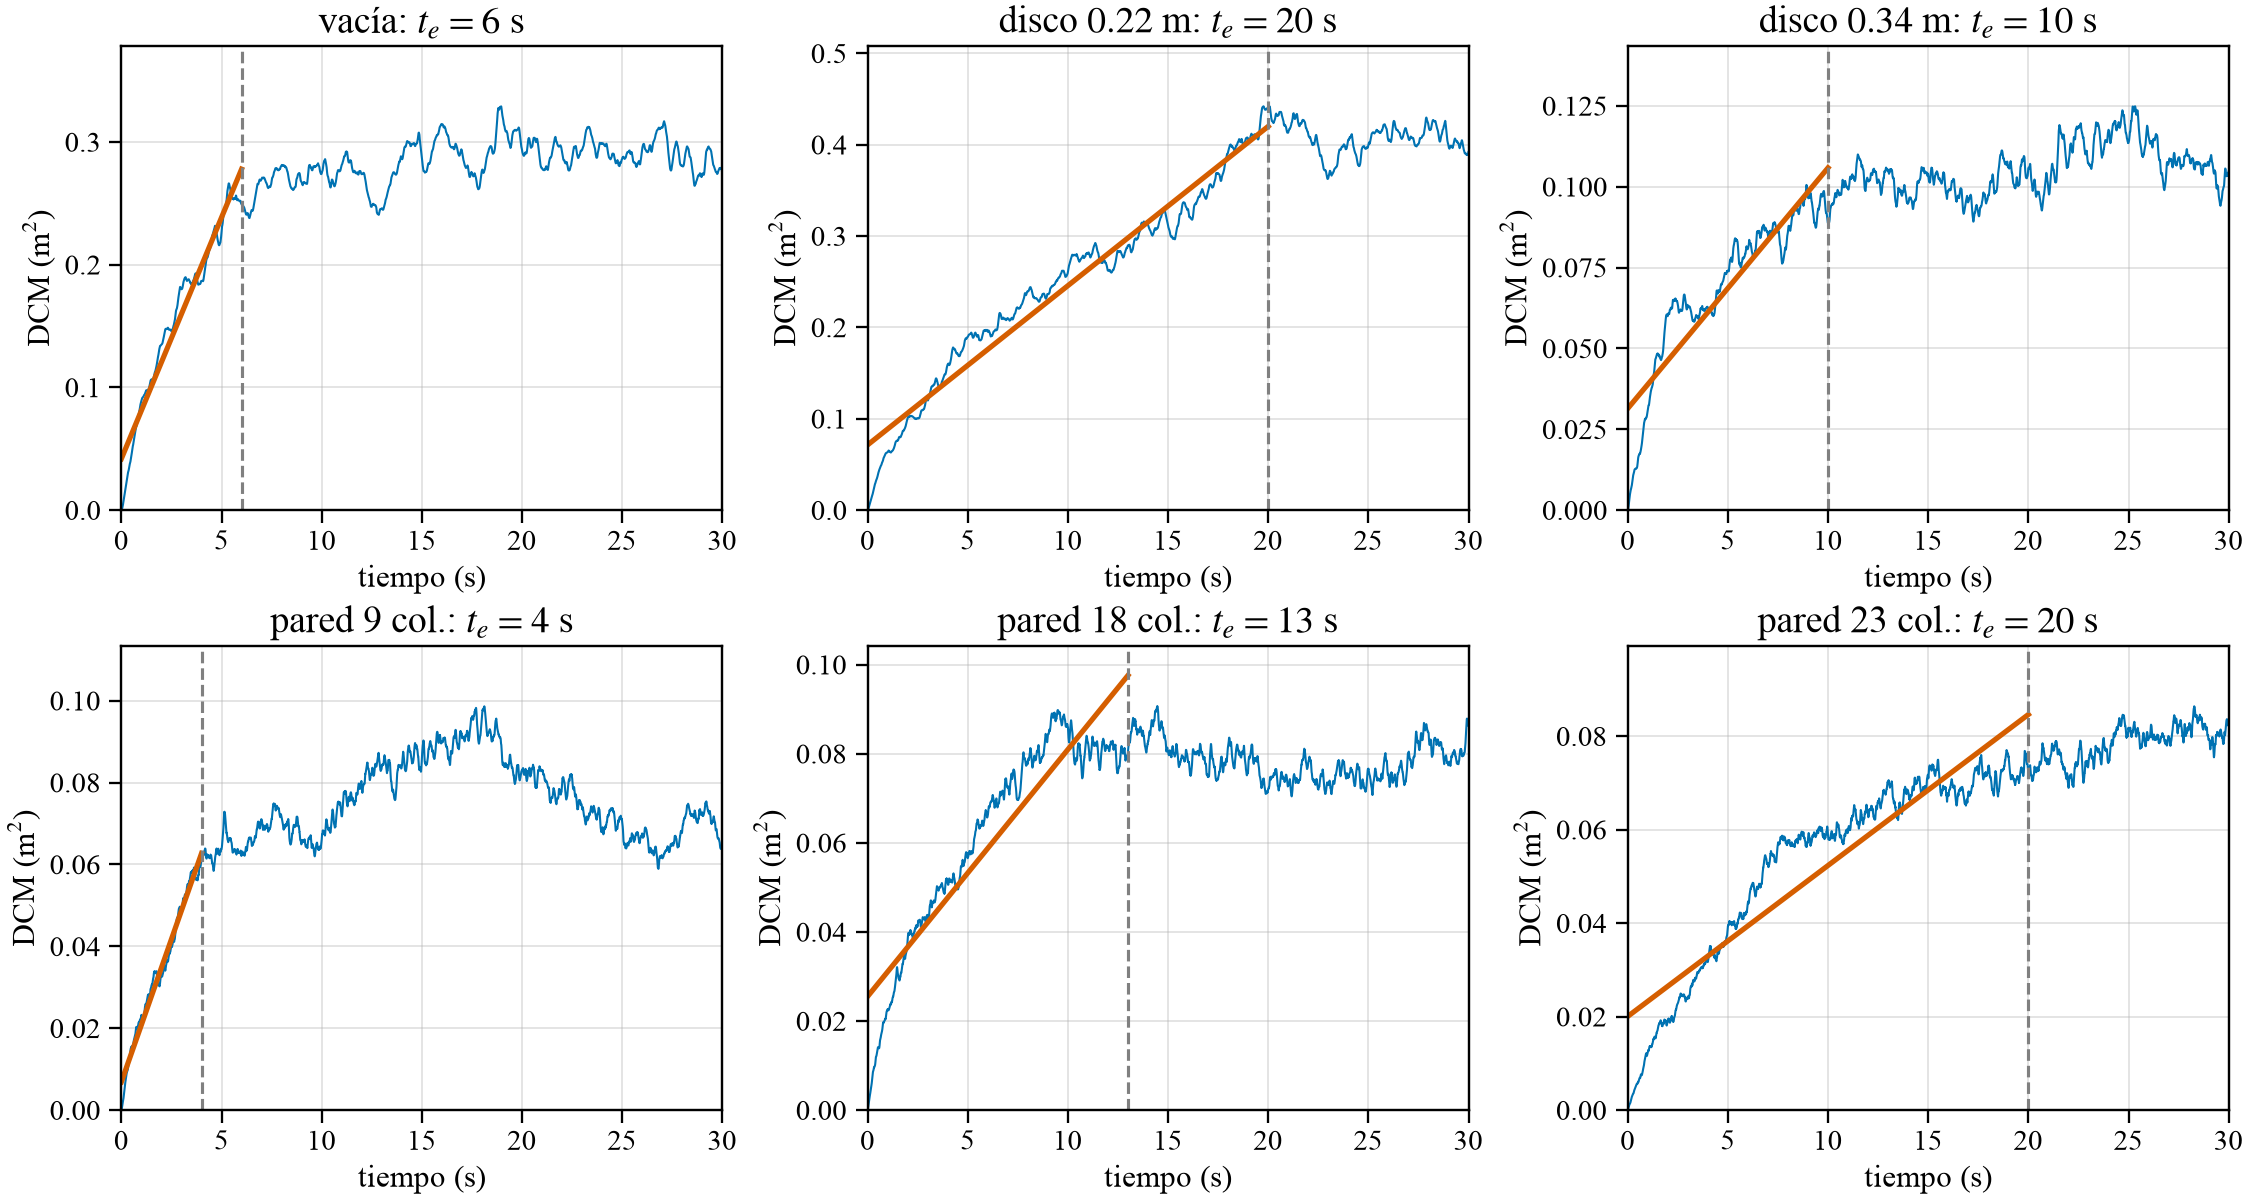
\includegraphics[width=\linewidth,height=0.8\textheight,keepaspectratio]{respaldo_te_configs.png}
  \par{\scriptsize Una realización (semilla 401). Punteada: $t_e$. Naranja: ajuste $4Dt + b$ en $[0, t_e]$.}
\end{frame}

\begin{frame}[noframenumbering]{Apéndice}
  \centering
  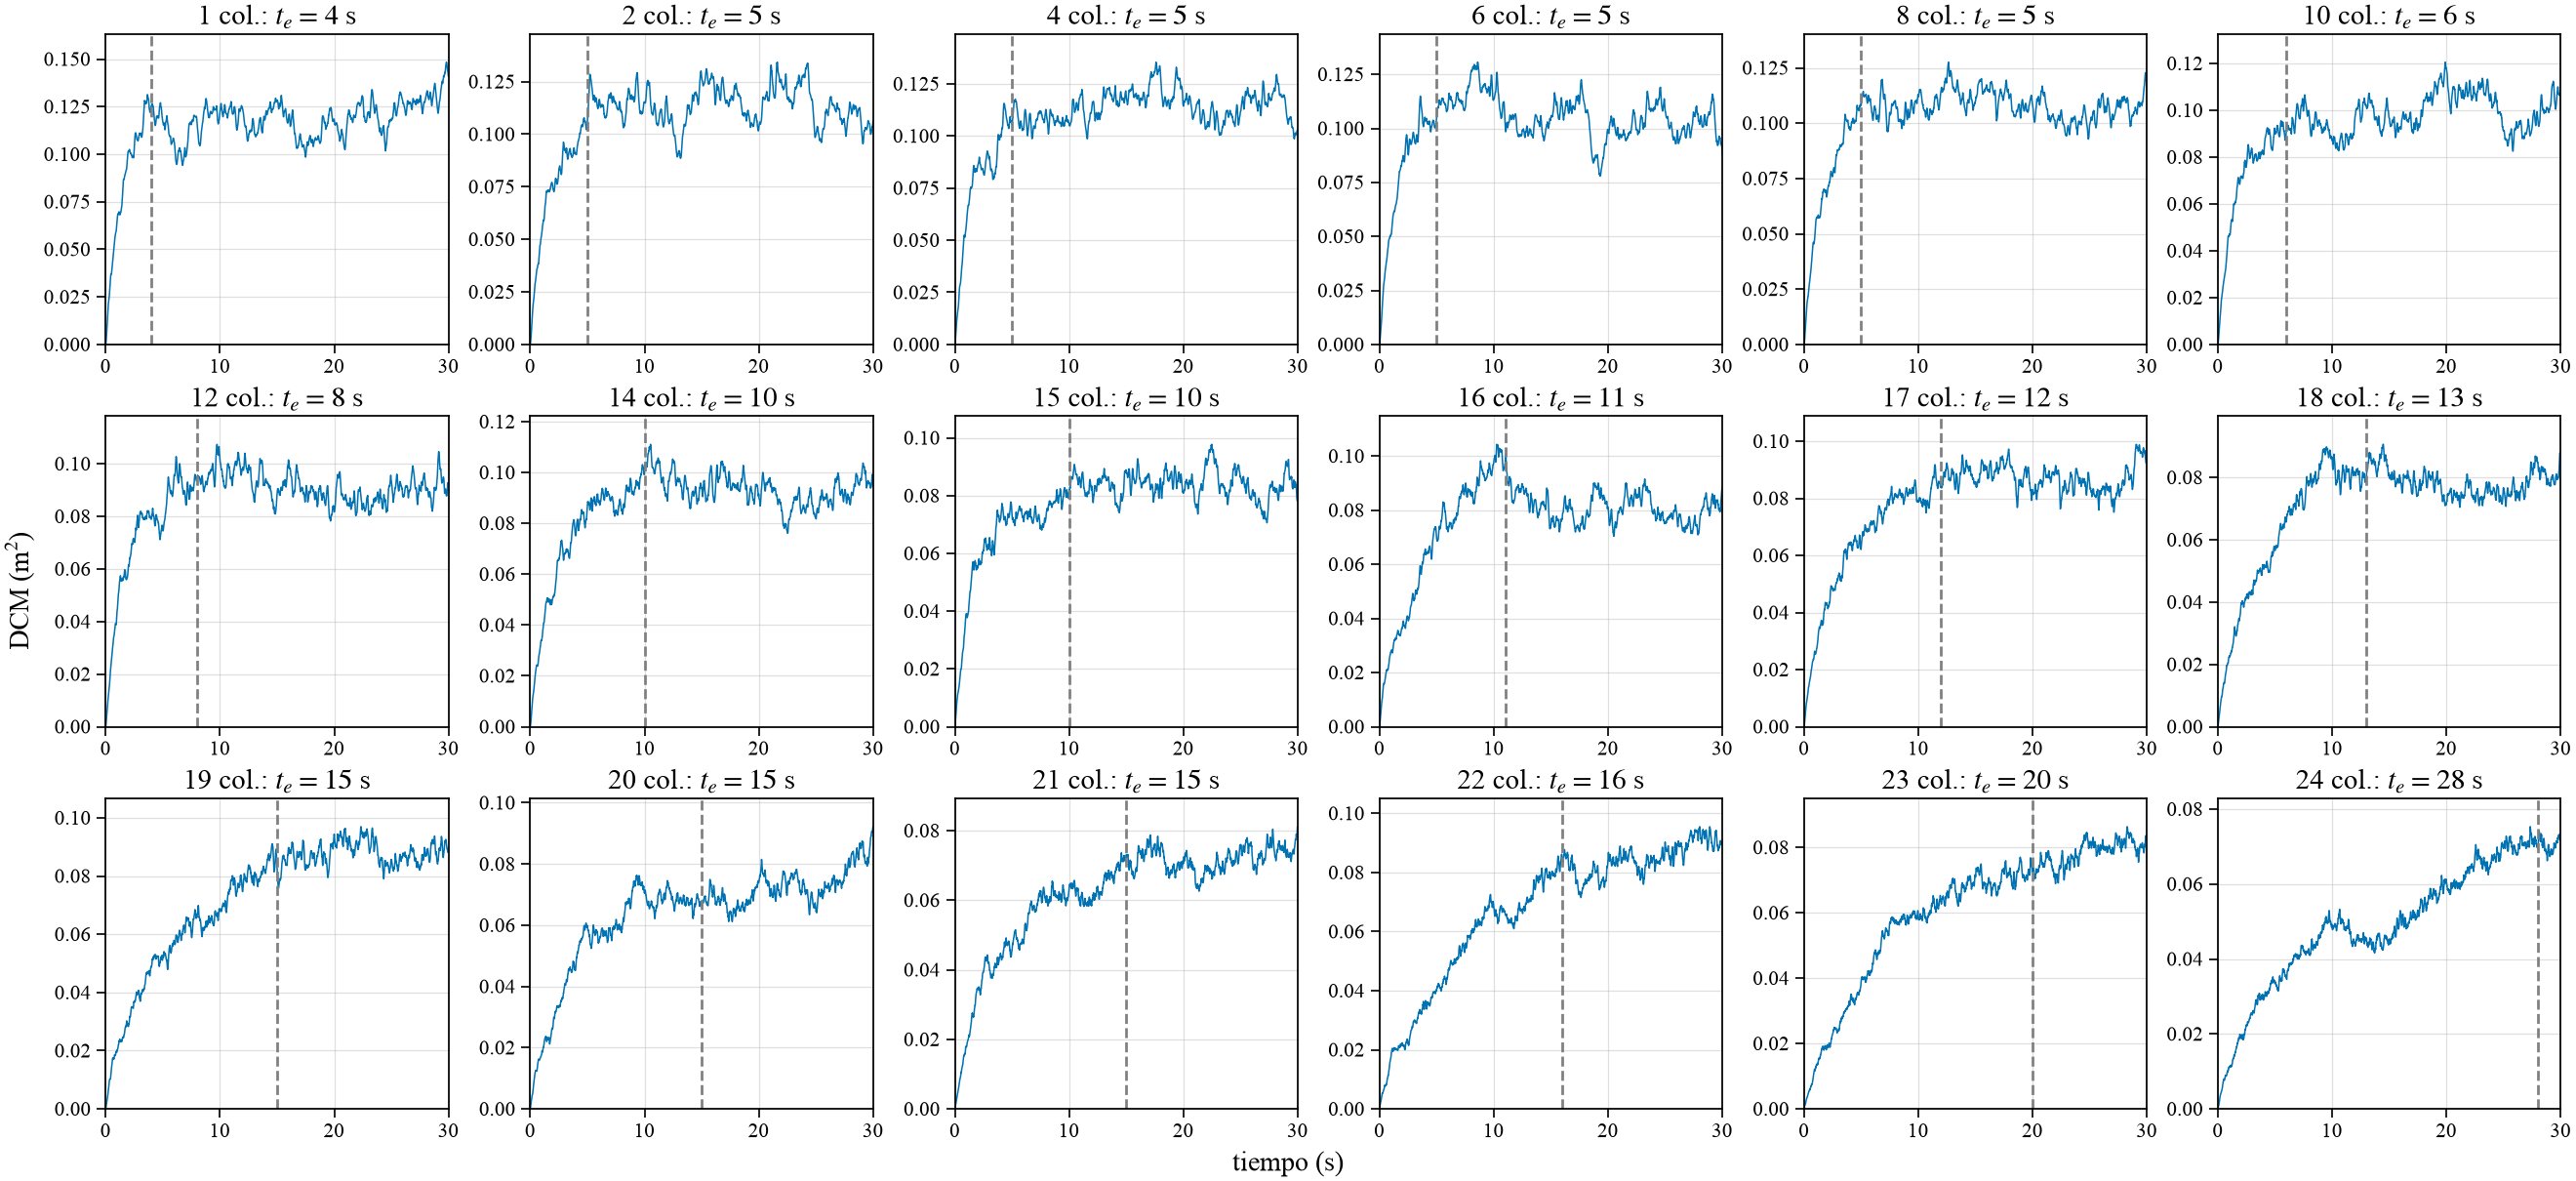
\includegraphics[width=\linewidth,height=0.8\textheight,keepaspectratio]{respaldo_te_barrido.png}
  \par{\scriptsize Una realización (semilla 401). Punteada: $t_e$.}
\end{frame}

\begin{frame}[noframenumbering]{Apéndice: $t_e$, $D$ y $\langle t_{90}\rangle$ en el barrido de columnas}
  \centering\scriptsize
  \renewcommand{\arraystretch}{1.2}
  \setlength{\tabcolsep}{4pt}
  % Generado por python/dcm_barrido.py (docs/results/1.3/cortes_barrido.txt). No editar a mano.
\begin{tabular}{cccc|cccc}
  \hline
  columnas & $t_e$ (s) & $D$ (m$^{2}$/s) & $\langle t_{90}\rangle$ (s) & columnas & $t_e$ (s) & $D$ (m$^{2}$/s) & $\langle t_{90}\rangle$ (s) \\
  \hline
  1 & $4$ & $0.0067 \pm 0.0006$ & $21.5 \pm 2.9$ & 16 & $11$ & $0.0015 \pm 0.0003$ & $15.0 \pm 1.5$ \\
  2 & $5$ & $0.0048 \pm 0.0008$ & $21.6 \pm 2.5$ & 17 & $12$ & $0.0013 \pm 0.0002$ & $14.8 \pm 1.6$ \\
  4 & $5$ & $0.0044 \pm 0.0005$ & $19.3 \pm 2.6$ & 18 & $13$ & $0.0013 \pm 0.0002$ & $13.7 \pm 1.3$ \\
  6 & $5$ & $0.0043 \pm 0.0003$ & $18.7 \pm 1.7$ & 19 & $15$ & $0.00104 \pm 0.00017$ & $13.9 \pm 2.0$ \\
  8 & $5$ & $0.0041 \pm 0.0007$ & $18.1 \pm 1.7$ & 20 & $15$ & $0.00105 \pm 0.00018$ & $14.3 \pm 1.5$ \\
  10 & $6$ & $0.0031 \pm 0.0005$ & $16.7 \pm 2.8$ & 21 & $15$ & $0.00105 \pm 0.00014$ & $14.5 \pm 0.8$ \\
  12 & $8$ & $0.0021 \pm 0.0003$ & $16.0 \pm 1.3$ & 22 & $16$ & $0.00099 \pm 0.00020$ & $15.7 \pm 1.9$ \\
  14 & $10$ & $0.0017 \pm 0.0002$ & $15.8 \pm 2.0$ & 23 & $20$ & $0.00077 \pm 0.00010$ & $17.0 \pm 1.7$ \\
  15 & $10$ & $0.00152 \pm 0.00018$ & $15.1 \pm 1.6$ & 24 & $28$ & $0.00055 \pm 0.00008$ & $18.6 \pm 2.3$ \\
  \hline
\end{tabular}

  \par\vspace{6pt}
  {$D$: promedio de $10$ realizaciones $\pm$ desvío estándar. Pared $R = r$, centro $x = 0.60\,\mathrm{m}$.}
\end{frame}

% Apéndice: las diapositivas del DCM repetidas con una ventana fija [0, 1 s] para todas
% (SHORT_WINDOW en python/dcm_report.py).
\begin{frame}[noframenumbering]{Apéndice $[0, 1\,\mathrm{s}]$: desplazamiento cuadrático medio}
  \begin{cols}
    \begin{column}{0.62\textwidth}
      \figura{respaldo_v1_vacia.png}
    \end{column}
    \begin{column}{0.34\textwidth}
      \begin{parametros}
        \item Mesa vacía, $N = 100$, semilla 401
        \item Ajuste de $4Dt + b$ en $[0, \DcmVentanaCorta\,\mathrm{s}]$, igual para todas
      \end{parametros}
      \begin{resultado}
        \item $D = \DcmDvaciaCorta\,\mathrm{m}^{2}/\mathrm{s}$
      \end{resultado}
      {\scriptsize $D$: promedio de los ajustes de $10$ realizaciones. En la principal, con $t_e$: $\DcmDvacia$.}
    \end{column}
  \end{cols}
\end{frame}

\begin{frame}[noframenumbering]{Apéndice $[0, 1\,\mathrm{s}]$: ajuste de $\langle \Delta r^{2}\rangle = 4Dt + b$}
  \begin{cols}
    \begin{column}{0.62\textwidth}
      \figura{respaldo_v1_error.png}
    \end{column}
    \begin{column}{0.34\textwidth}
      \begin{parametros}
        \item Puntos en $[0, \DcmVentanaCorta\,\mathrm{s}]$ de una realización
        \item Semilla 401
      \end{parametros}
      \begin{resultado}
        \item $D^{*} = \DcmDejemploCorta\,\mathrm{m}^{2}/\mathrm{s}$
      \end{resultado}
    \end{column}
  \end{cols}
\end{frame}

\begin{frame}[noframenumbering]{Apéndice $[0, 1\,\mathrm{s}]$: DCM según la configuración}
  \begin{cols}
    \begin{column}{0.62\textwidth}
      \figura{respaldo_v1_configs.png}
    \end{column}
    \begin{column}{0.34\textwidth}
      \begin{parametros}
        \item Primeros $2\,\mathrm{s}$, una realización (semilla 401)
        \item Punteada: fin de la ventana
      \end{parametros}
      \begin{resultado}
        \item Mismos dos grupos que en $30\,\mathrm{s}$
      \end{resultado}
    \end{column}
  \end{cols}
\end{frame}

\begin{frame}[noframenumbering]{Apéndice $[0, 1\,\mathrm{s}]$: $D$ y $\langle t_{90}\rangle$}
  \centering\small
  \renewcommand{\arraystretch}{1.3}
  % Generado por python/dcm_report.py (docs/results/1.3/cortes.txt). No editar a mano.
\begin{tabular}{lcccc}
  \hline
  configuración & área ocupada & $D$, $[0, t_e]$ & $D$, $[0, 1\,\mathrm{s}]$ & $\langle t_{90}\rangle$ (s) \\
  \hline
  mesa vacía & 0\,\% & $0.0093 \pm 0.0014$ & $0.024 \pm 0.003$ & $24 \pm 3$ \\
  disco, $R = 0.22\,\mathrm{m}$ & 19\,\% & $0.0032 \pm 0.0007$ & $0.015 \pm 0.003$ & $20 \pm 3$ \\
  pared, 9 columnas & 38\,\% & $0.0030 \pm 0.0005$ & $0.0058 \pm 0.0007$ & $14.2 \pm 1.4$ \\
  disco, $R = 0.34\,\mathrm{m}$ & 45\,\% & $0.0020 \pm 0.0002$ & $0.0070 \pm 0.0010$ & $17.0 \pm 2.0$ \\
  pared, 18 columnas & 40\,\% & $0.0013 \pm 0.0002$ & $0.0065 \pm 0.0008$ & $13.7 \pm 1.3$ \\
  pared, 23 columnas & 52\,\% & $0.00077 \pm 0.00010$ & $0.0028 \pm 0.0003$ & $17.0 \pm 1.7$ \\
  \hline
\end{tabular}

  \par\vspace{8pt}
  {\footnotesize Mismas $10$ realizaciones. Con $[0, 1\,\mathrm{s}]$ los valores son mayores (incluye el vuelo libre inicial),
  pero la tendencia se mantiene: mayor $D$ en la mesa vacía, menor con más área ocupada.}
\end{frame}

\begin{frame}[noframenumbering]{Apéndice $[0, 1\,\mathrm{s}]$: $\langle t_{90}\rangle$ y $D$ según las columnas}
  \begin{cols}
    \begin{column}{0.62\textwidth}
      \figura{respaldo_v1_columnas.png}
    \end{column}
    \begin{column}{0.34\textwidth}
      \begin{parametros}
        \item Pared $R = r$, centro $x = 0.60\,\mathrm{m}$
        \item Línea punteada: 18 columnas
      \end{parametros}
      \begin{resultado}
        \item $D$ baja al agregar columnas
        \item $\langle t_{90}\rangle$ mínimo en 18 columnas
      \end{resultado}
    \end{column}
  \end{cols}
\end{frame}

\begin{frame}[noframenumbering]{Apéndice: $D$ con las dos ventanas en el barrido de columnas}
  \begin{cols}
    \begin{column}{0.62\textwidth}
      \figura{respaldo_ventana_barrido.png}
    \end{column}
    \begin{column}{0.34\textwidth}
      \begin{parametros}
        \item Pared $R = r$, centro $x = 0.60\,\mathrm{m}$
        \item Punteada: 18 columnas
      \end{parametros}
      \begin{resultado}
        \item Con las dos ventanas, $D$ baja al agregar columnas
      \end{resultado}
    \end{column}
  \end{cols}
\end{frame}

\end{document}
